% !TeX root = index.tex
\documentclass[a4paper, 12pt]{report}		% general format

%%%% Charset
\usepackage{cmap}							% make PDF files searchable and copyable
\usepackage[utf8]{inputenc}					% accept different input encodings
\usepackage[T2A]{fontenc}					% russian font
\usepackage[russian]{babel}					% multilingual support (T2A)

%%%% Graphics
\usepackage[dvipsnames]{xcolor}			% driver-independent color extensions
\usepackage{graphicx}						% enhanced support for graphics
\usepackage{wrapfig}						% pro­duces fig­ures which text can flow around

%%%% Math
\usepackage{amsmath}						% Amer­i­can Math­e­mat­i­cal So­ci­ety (AMS) math fa­cil­i­ties
\usepackage{amsfonts}						% fonts from the AMS
\usepackage{amssymb}						% additional math symbols

%%%% Ty­po­grapy (don't forget about cm-super)
\usepackage{microtype}						% sublim­i­nal re­fine­ments to­wards ty­po­graph­i­cal per­fec­tion
\linespread{1.3}							% line spacing
\usepackage[left=2.5cm, right=1.5cm, top=2.5cm, bottom=2.5cm]{geometry}
\setlength{\parindent}{0pt}					% we don't want any paragraph indentation
\setlength{\parskip}{0.3cm}
\renewcommand{\chaptername}{}

%%%% Other
\usepackage{hyperref}							% ver­ba­tim with URL-sen­si­tive line breaks
\usepackage{fancyvrb}
%\DeclareUnicodeCharacter{00A0}{~}
\usepackage{float}
\usepackage{color,soul}

%------------------------------------------------------------------------------
\usepackage{listings}						% type­set source code list­ings

% Цвета для кода
\definecolor{string}{HTML}{101AF9}			% цвет строк в коде
\definecolor{comment}{HTML}{3F7F5F}		% цвет комментариев в коде
\definecolor{keyword}{HTML}{5F1441}		% цвет ключевых слов в коде
\definecolor{morecomment}{HTML}{8000FF}	% цвет include и других элементов в коде
\definecolor{captiontext}{HTML}{FFFFFF}	% цвет текста заголовка в коде
\definecolor{captionbk}{HTML}{999999}		% цвет фона заголовка в коде
\definecolor{bk}{HTML}{FFFFFF}				% цвет фона в коде
\definecolor{frame}{HTML}{999999}			% цвет рамки в коде

% Настройки отображения кода
\lstset{
	language=C++,							% Язык кода по умолчанию
	morekeywords={*,...},					% если хотите добавить ключевые слова, то добавляйте
	% Цвета
	keywordstyle=\color{keyword}\ttfamily\bfseries,
	stringstyle=\color{string}\ttfamily,
	commentstyle=\color{comment}\ttfamily\itshape,
	morecomment=[l][\color{morecomment}]{\#},
	% Настройки отображения
	breaklines=true,						% Перенос длинных строк
	basicstyle=\ttfamily\footnotesize,		% Шрифт для отображения кода
	backgroundcolor=\color{bk},				% Цвет фона кода
	%frame=lrb,xleftmargin=\fboxsep,xrightmargin=-\fboxsep, % Рамка, подогнанная к заголовку
	frame=tblr								% draw a frame at all sides of the code block
	rulecolor=\color{frame},				% Цвет рамки
	tabsize=2,								% tab space width
	showstringspaces=false,					% don't mark spaces in strings
	% Настройка отображения номеров строк. Если не нужно, то удалите весь блок
	numbers=left,							% Слева отображаются номера строк
	stepnumber=1,							% Каждую строку нумеровать
	numbersep=5pt,							% Отступ от кода
	numberstyle=\small\color{black},		% Стиль написания номеров строк
	% Для отображения русского языка
	extendedchars=true,
    literate=
        {Ö}{{\"O}}1                    {Ä}{{\"A}}1                    {Ü}{{\"U}}1
        {ß}{{\ss}}1                    {ü}{{\"u}}1                    {ä}{{\"a}}1
        {ö}{{\"o}}1                    {~}{{\textasciitilde}}1        {а}{{\selectfont\char224}}1
        {б}{{\selectfont\char225}}1    {в}{{\selectfont\char226}}1    {г}{{\selectfont\char227}}1
        {д}{{\selectfont\char228}}1    {е}{{\selectfont\char229}}1    {ё}{{\"e}}1
        {ж}{{\selectfont\char230}}1    {з}{{\selectfont\char231}}1    {и}{{\selectfont\char232}}1
        {й}{{\selectfont\char233}}1    {к}{{\selectfont\char234}}1    {л}{{\selectfont\char235}}1
        {м}{{\selectfont\char236}}1    {н}{{\selectfont\char237}}1    {о}{{\selectfont\char238}}1
        {п}{{\selectfont\char239}}1    {р}{{\selectfont\char240}}1    {с}{{\selectfont\char241}}1
        {т}{{\selectfont\char242}}1    {у}{{\selectfont\char243}}1    {ф}{{\selectfont\char244}}1
        {х}{{\selectfont\char245}}1    {ц}{{\selectfont\char246}}1    {ч}{{\selectfont\char247}}1
        {ш}{{\selectfont\char248}}1    {щ}{{\selectfont\char249}}1    {ъ}{{\selectfont\char250}}1
        {ы}{{\selectfont\char251}}1    {ь}{{\selectfont\char252}}1    {э}{{\selectfont\char253}}1
        {ю}{{\selectfont\char254}}1    {я}{{\selectfont\char255}}1    {А}{{\selectfont\char192}}1
        {Б}{{\selectfont\char193}}1    {В}{{\selectfont\char194}}1    {Г}{{\selectfont\char195}}1
        {Д}{{\selectfont\char196}}1    {Е}{{\selectfont\char197}}1    {Ё}{{\"E}}1
        {Ж}{{\selectfont\char198}}1    {З}{{\selectfont\char199}}1    {И}{{\selectfont\char200}}1
        {Й}{{\selectfont\char201}}1    {К}{{\selectfont\char202}}1    {Л}{{\selectfont\char203}}1
        {М}{{\selectfont\char204}}1    {Н}{{\selectfont\char205}}1    {О}{{\selectfont\char206}}1
        {П}{{\selectfont\char207}}1    {Р}{{\selectfont\char208}}1    {С}{{\selectfont\char209}}1
        {Т}{{\selectfont\char210}}1    {У}{{\selectfont\char211}}1    {Ф}{{\selectfont\char212}}1
        {Х}{{\selectfont\char213}}1    {Ц}{{\selectfont\char214}}1    {Ч}{{\selectfont\char215}}1
        {Ш}{{\selectfont\char216}}1    {Щ}{{\selectfont\char217}}1    {Ъ}{{\selectfont\char218}}1
        {Ы}{{\selectfont\char219}}1    {Ь}{{\selectfont\char220}}1    {Э}{{\selectfont\char221}}1
        {Ю}{{\selectfont\char222}}1    {Я}{{\selectfont\char223}}1    {і}{{\selectfont\char105}}1
        {ї}{{\selectfont\char168}}1    {є}{{\selectfont\char185}}1    {ґ}{{\selectfont\char160}}1
        {І}{{\selectfont\char73}}1     {Ї}{{\selectfont\char136}}1    {Є}{{\selectfont\char153}}1
        {Ґ}{{\selectfont\char128}}1
}

% Для настройки заголовка кода
\usepackage{caption}
\DeclareCaptionFont{white}{\color{сaptiontext}}
\DeclareCaptionFormat{listing}{\parbox{\linewidth}{\colorbox{сaptionbk}{\parbox{\linewidth}{#1#2#3}}\vskip-4pt}}
%\captionsetup[lstlisting]{format=listing,labelfont=white,textfont=white}
\renewcommand{\lstlistingname}{Листинг} % Переименование Listings в нужное именование структуры

%------------------------------------------------------------------------------
\begin{document}

\begin{titlepage}

%----------------------------------------------------------------------------------------
%	HEADING SECTIONS
%----------------------------------------------------------------------------------------
\begin{center} % Center everything
Федеральное государственное автономное образовательное \\
учреждение высшего образования \\[0.4cm]
% https://www.spbstu.ru/university/organizational-documents/corporate-identity/

\includegraphics[scale=0.8]{res/SPbPU-logo} \\[0.4cm]
Институт компьютерных наук и технологий \\*
Высшая школа интеллектуальных систем и суперкомпьютерных технологий
\end{center}

\vspace{3cm}

%----------------------------------------------------------------------------------------
%	TITLE SECTION
%----------------------------------------------------------------------------------------
\begin{center} % Center everything
\textbf{Курсовая работа}\\
по дисциплине "Сетевая безопасность"\\
на тему\\
\textbf{Исследование коммуникационного протокола WebSocket}
\end{center}

\vspace{3.5cm}
 
%----------------------------------------------------------------------------------------
%	AUTHOR SECTION
%----------------------------------------------------------------------------------------
\begin{flushleft}
Выполнил студент гр. 3540901/21501 \hspace{3cm} $\underset{\text{(подпись)}}{\underline{\hspace{3cm}}}$ С.А.Мартынов\\[0.5cm]
Преподаватель \hspace{7.25cm} $\underset{\text{(подпись)}}{\underline{\hspace{3cm}}}$ В.Э. Шмаков\\[0.5cm]
\hspace{10.2cm} «\underline{\hspace{1cm}}» \underline{\hspace{3cm}} 2023 г.
\end{flushleft}

\vfill % Fill the rest of the page with whitespace

%----------------------------------------------------------------------------------------
%	DATE SECTION
%----------------------------------------------------------------------------------------
\begin{center}
Санкт-Петербург\\
2023
\end{center}

\end{titlepage}

\setcounter{page}{2}                            % inclide the title page
\tableofcontents
\chapter*{Лабораторная работа 1. Сокетные соединения}
\addcontentsline{toc}{chapter}{Лабораторная работа 1. Сокетные соединения}

\textbf{Цель работы:} Освоение набора системных вызовов для создания сокетных соединений различных типов, для обмена данными на хостах и по сети.

\section*{1. Системные вызовы}
\textbf{Задача:} Проанализируйте набор системных вызовов для серверной и клиентской сторон при организации соединений на сокетах под ОС Linux, принимая во внимание возможности различных видов сокетов и семейств адресации.

\textbf{Ход решения:}

Основные вызовы:
\begin{itemize}
    \item \texttt{socket()} -- создать новый сокет и вернуть файловый дескриптор;
    \item \texttt{send()} -- отправить данные по сети;
    \item \texttt{receive()} -- получить данные из сети;
    \item \texttt{close()} -- закрыть соединение.
\end{itemize}

Основные вызовы на стороне сервера:
\begin{itemize}
    \item \texttt{bind()} -- связать сокет с IP-адресом и портом;
    \item \texttt{listen()} -- слушает порт и ждет когда будет установлено соединение;
    \item \texttt{accept()} -- принять запрос на установку соединения.
\end{itemize}

Основные вызовы на стороне клиента:
\begin{itemize}
    \item \texttt{connect()} -- установить соединение.
\end{itemize}

Основные семейства протоколов создаваемого сокета:
\begin{itemize}
    \item \texttt{AF\_INET} -- для сетевого протокола IPv4;
    \item \texttt{AF\_INET6} -- для IPv6;
    \item \texttt{AF\_UNIX} -- для локальных сокетов (используя файл).
\end{itemize}

Основные типы соединений:
\begin{itemize}
    \item \texttt{SOCK\_STREAM} -- надёжная потокоориентированная служба или потоковый сокет;
    \item \texttt{SOCK\_DGRAM} -- служба датаграмм или датаграммный сокет;
    \item \texttt{SOCK\_RAW} -- сырой протокол поверх сетевого уровня.
\end{itemize}

\section*{2. Присоединенные сокеты}
\textbf{Задача:} Скомпилируйте и выполните программу \texttt{socketpair.cpp}, иллюстрирующую создание простейшего вида сокета и обмен данными двух родственных процессов.

Проанализируйте вывод на консоль. Существует ли зависимость обмена от различных соотношений величин временных задержек (в вызовах \texttt{sleep()}) в процессе-родителе и в процессе-потомке?

\textbf{Ход решения:} Беглый анализ исходного текста позволяет выявить следующие моменты:
\begin{enumerate}
    \item{В цикле \texttt{switch} дан не правильный комментарий для поведения по умолчанию: там сказано, что дальнейший код будет исполняться потомком, хотя это не так. Системный вызов \texttt{fork()} возвращает положительное не нулевое число для процесса-родителя.}
    \item{Для организации сетевого взаимодействия используется системный вызов \texttt{socketpair()}, который создает пару безымянных присоединённых сокетов. Рассмотрим параметры, которые используются для этого системного вызова:
                \begin{itemize}
                    \item \texttt{PF\_UNIX} показывает, что будет использовано локальное соединение.
                    \item \texttt{SOCK\_STREAM} показывает, что семантика коммуникации обеспечивает создание двусторонних надежных и последовательных потоков байтов, поддерживающих соединения.
                \end{itemize}
                Остальные параметры тривиальны.
          }
    \item{Учитывая, что потомок всегда пишет, и только потом читает, а предок действует наоборот, и при этом у нас блокирующие операции, сразу понятно, что будет простой поочерёдный обмен, и вызов \texttt{sleep()} ни на что не влияет. Или, другими словами, каждый этот вызов будет влиять и на одну и на другую сторону общения, увеличивая их ожидание.}
\end{enumerate}

\textbf{Эксперимент:} Запустив приложение, мы получили следующий вывод:
\begin{Verbatim}[frame=single]
    smart@thinkpad$ ./socketpair
    p->c:0
    c->p: 1
    p->c:2
    c->p: 3
    p->c:4
    c->p: 5
    p->c:6
    c->p: 7
    p->c:8
    c->p: 9
\end{Verbatim}

Дальнейшие эксперименты с \texttt{sleep()} подтвердили изначальные гипотезы: можно полностью убрать оба вызова \texttt{sleep()} и это не сломает программу, можно увеличивать значение параметра для \texttt{sleep()} и это будет влиять на оба процесса.

\section*{3. Локальные сокеты}
\textbf{Задача:} Скомпилируйте программы \texttt{echo\_server.cpp} и \texttt{echo\_client.cpp}, задавая им при компиляции разные имена.

Запустите программы сервера и клиента на разных терминалах. Введите символьную информацию в окне клиента и проанализируйте вывод. Какой разновидности принадлежат сокеты, используемые в данном примере клиент-серверного взаимодействия?

С чем связано создание специального файла в текущем каталоге во время исполнения программ?

\textbf{Ход решения:} Начнём с анализа исходных кодов.

Сервер:
\begin{enumerate}
\item Создаётся сокет, используя системный вызов \texttt{socket()}. Параметры \texttt{AF\_UNIX} и \texttt{SOCK\_STREAM} идентичны параметрам из предыдущего шага (\texttt{AF\_UNIX} это синоним для \texttt{PF\_UNIX}). Фактический результат этого вызова -- файловый дескриптор.
\item Для соединения (\texttt{bind()}) сокета с адресом (\texttt{sockaddr\_un}), производится подготовка этого адреса. Обычно тут задаётся адрес хоста и номер порта для ожидания соединения, но в данном случае адресу задаётся семейство, идентичное семейству сокета (\texttt{AF\_UNIX}) и указывается путь, где сокет будет располагаться в файловой системе. Вызов (\texttt{unlink()}) позволяет автоматически удалить файл сокета, когда он перестанет использоваться.
\item После связывания, сокет переводится в режим прослушивания (\texttt{listen()}). Число 5 позволяет размер очереди клиентов, желающих подключиться.
\item В бесконечном цикле, сервер ожидает подключения клиента. Исполнение процесса будет заблокировано на вызове \texttt{accept()}. Этот вызов позволяет позволяет получить копию исходного сокета, чтобы слушающий сокет был готов к получению запросов от других клиентов.
\item После этого снова в бесконечном цикле происходит получение и отправка сообщений длинной в 100 символов через копию сокета, полученного на предыдущем шаге.
\end{enumerate}

клиент:
\begin{enumerate}
\item Подобно серверу, создаётся сокет, используя системный вызов \texttt{socket()} с параметрами \texttt{AF\_UNIX} и \texttt{SOCK\_STREAM}.
\item На клиенте идёт подготовка к соединению. Обычно используется имя удалённого хоста и номер порта. Однако в нашем случае используется адрес сокета в файловой системе (адрес записывается в структуру \texttt{sockaddr\_un}).
\item Дальше следует непосредственно соединение (\texttt{connect()}).
\item В бесконечном цикле происходит считывание данных с устройства ввода (\texttt{stdin}), отправка их серверу, получение ответа от сервера и вывод этого ответа на стандартное устройство вывода (\texttt{stdout}).
\end{enumerate}

\textbf{Эксперимент:} Запуск сервера:
\begin{Verbatim}[frame=single]
    smart@thinkpad$ ./echo_server
    Waiting for a connection...
\end{Verbatim}

Запуск клиента:
\begin{Verbatim}[frame=single]
    smart@thinkpad$ ./echo_client
    Trying to connect...
    Connected.
    > 123
    echo> 123
    > test
    echo> test
    > тест
    echo> тест
    > ~!@#$%
    echo> ~!@#$%
    > 
\end{Verbatim}

После запуска сервера, в директории появляется файл сокета. Инормацию о нём можно получить, к примеру, с помощью утилиты \texttt{ss}.
\begin{Verbatim}[frame=single]
smart@thinkpad$ ss | grep echo_socket
u_str ESTAB    0      0               echo_socket 481033            * 481088
\end{Verbatim}
Эта запись означает следующее:
\begin{itemize}
    \item \texttt{u\_str} -- сетевой идентификатор;
    \item \texttt{ESTAB} -- состояние соединения;
    \item 0 -- количество пакетов в очереди на получение (\texttt{Recv-Q});
    \item 0 -- количество пакетов в очереди на отправку (\texttt{Send-Q});
    \item echo\_socket 481033 -- локальный адрес и порт (большое число для локальных соединений);
    \item $\ast{}$ 481088 -- адрес и порт клиента.
\end{itemize}

\section*{4. Интернет сокеты}
\textbf{Задача:} Скомпилируйте c разными именами программы \texttt{sock\_c\_i\_srv.cpp} и \texttt{sock\_c\_i\_clt.cpp} (в них используется общий \texttt{include} файл \texttt{local\_c\_i.h}). Запустите программы сервера и клиента на разных терминалах. При запуске клиента указывайте в качестве параметра командной строки имя хоста \texttt{localhost}. Введите символьную информацию в окне клиента и поясните вывод.

Какой разновидности принадлежат сокеты, используемые в данном примере клиент-серверного взаимодействия?

\textbf{Ход решения:} Проведём анализ кода. Алгоритм практически аналогичен предыдущему примеру, но тут используется семейство \texttt{AF\_INET} и создание отдельных процессов для обслуживания клиентов. В данном примере, мы как и раньше используем потоковую передачу (\texttt{SOCK\_STREAM}), однако сетевые сокеты позволяют организовать передачу на датаграммах (\texttt{SOCK\_STREAM}) -- такие соединения работают без подтверждения факта доставки (\texttt{ACK}).

И сервер и клиент при вызове функции \texttt{socket()} используют константу \texttt{AF\_INET}, указывающую на то, что открываемый сокет должен быть сетевым. Сокеты в домене \texttt{AF\_INET}, не знают про то, что они работают на локальной системе и обращаются только к \texttt{localhost}. Они полностью выполняют все механизмы сетевого стека: переключения контекста, \texttt{ACK}, \texttt{TCP}, управление потоком, маршрутизацию, разбиение больших пакетов и т.п. То есть это «полноценная TCP работа» несмотря на то, что пакеты не покидают локального интерфейса.

Дополнительные издержки при использовании \texttt{AF\_INET} кроются так же в необходимости произвести резолвинг доменного имени в IP-адрес (вызов \texttt{gethostbyname()}) и решение проблемы little-big-end (вызов \texttt{htons()}, \texttt{htonl()}) связанной с разным порядком байтов на различных архитектурах (в комментариях кода написано что-то странное про "fake port").

Ещё одной особенность является обработка подключений клиентов в отдельных процессах. После установки соединения, сервер вызывает \texttt{fork()} и работает с каждым клиентом отдельно. Это значит, что каждый клиент получит в ответ только свои сообщения.

\textbf{Эксперимент:} запуск сервера.
\begin{Verbatim}[frame=single]
    smart@thinkpad$ ./sock_c_i_srv 
\end{Verbatim}

Запуск первого клиента.
\begin{Verbatim}[frame=single]
    smart@thinkpad$ ./sock_c_i_clt localhost
    > 1
    1
    > 2
    2
    > 3
    3
    > 
\end{Verbatim}

Запуск второго клиента.
\begin{Verbatim}[frame=single]
    smart@thinkpad$ ./sock_c_i_clt localhost
    > a
    A
    > b
    B
    > c
    C
    > d
    D
    > 
\end{Verbatim}

Замена строчных букв на заглавные происходит на стороне сервера при помощи команды \texttt{toupper(buf[i])}.

\section*{5. Модификация эхо-сервера}
\textbf{Задача:} Модифицируйте программу \texttt{echo\_server.cpp} так, чтобы при ответе на запросы клиента что-либо выводилось в окне сервера.

Испытайте работу эхо-сервера при работе с несколькими клиентами.

\textbf{Ход решения:}

Фактически, была добавлена только строчка 3, представленная в листинге 1.

\lstinputlisting[language=C++, caption={Фрагмент исходного кода модифицированного файла (echo\_server\_upd.cpp)}, firstline=69, lastline=79]
{../Tasks/1_Network_application/source_files/echo_server_upd.cpp}

\textbf{Эксперимент:} запуск сервера.
\begin{Verbatim}[frame=single]
    smart@thinkpad$ ./echo_server_upd 
    Waiting for a connection...
    Connected.
    [client 4] 1
    [client 4] 2
    [client 4] 3
    [client 4] 4
    Waiting for a connection...
    Connected.
    [client 4] a
    [client 4] b
    [client 4] c
    [client 4] d
\end{Verbatim}

Запуск первого клиента.
\begin{Verbatim}[frame=single]
    smart@thinkpad$ ./echo_client 
    Trying to connect...
    Connected.
    > 1
    echo> 1
    > 2
    echo> 2
    > 3
    echo> 3
    > 4
    echo> 4
    > ^C
\end{Verbatim}

Запуск второго клиента.
\begin{Verbatim}[frame=single]
    smart@thinkpad$ ./echo_client 
    Trying to connect...
    Connected.
    > a
    b
    c
    d
    echo> a
    > echo> b
    > echo> c
    > echo> d
    > 
\end{Verbatim}

Наблюдаемое поведение полностью в рамках ожиданий: когда сервер установил соединение с первым клиентом, он находится в заблокированном состоянии на операции сетевого обмена. Как только первый клиент завершает свою работу, мгновенно происходит подключение и обслуживание второго клиента (он даже получает тот-же номер файлового дескриптора). Отсюда напрашивается вывод, что работа слушающего сокета должна производиться в одном потоке, а обслуживающих -- в другом (других).
\chapter*{Лабораторная работа 2. Сокеты L4}
\addcontentsline{toc}{chapter}{Лабораторная работа 2. Сокеты L4}

\textbf{Цель работы:} Создание клиент-серверных приложений, взаимодействующих друг с другом по сети на основе технологии соединения на сокетах L4.

\section*{1. Анализ кода}
\textbf{Задача:} Проанализируйте код программы \texttt{server\_game.cpp}, иллюстрирующей обмен данными с клиентскими приложениями по итеративной схеме.

\textbf{Ход решения:} Используется сокет семейства \texttt{AF\_INET}. Сервер ожидает соединения на любом IP адресе (\texttt{INADDR\_ANY}), но нам достаточно для подключения \texttt{localhost}. Для соединения будет использоваться порт 1066. Игра работает в один поток.

\section*{2. Компиляция и запуск}
\textbf{Задача:} Скомпилируйте и запустите \texttt{server\_game}.

\textbf{Эксперимент:} запуск сервера.
\begin{Verbatim}[frame=single]
    smart@thinkpad$ g++ server_game.cpp -o server_game
    smart@thinkpad$ ./server_game 
    start to listen

\end{Verbatim}

Системный журнал зафиксировал выбор слова сервером.
\begin{Verbatim}[frame=single]
    smart@thinkpad$ journalctl -a | grep server_game
    Feb 08 23:43:25 thinkpad server_game[103180]: server_game chose word green
    Feb 08 23:43:40 thinkpad server_game[103180]: server_game chose word green
\end{Verbatim}

\section*{3. Анализ состояния сокета}
\textbf{Задача:} Запустите другой терминал и проверьте с него наличие в системе созданного сервером сокета и то, что он находится в состоянии \texttt{LISTEN}. Для этого выполните команду \texttt{netstat -a | grep 1066}.

Проанализируйте вывод данной команды и объясните ее смысл.

\textbf{Ход решения:} Так как команда \texttt{netstat} устарела и была заменена на \texttt{ss}, то будет рассматривать вывод \texttt{ss -atp | grep game}

\textbf{Эксперимент:} результат запуска команды \texttt{ss}
\begin{Verbatim}[frame=single]
    smart@thinkpad$ ss -atp | grep game
    State  Recv-Q Send-Q Local Address:Port       Peer Address:PortProcess
    LISTEN 0      5            0.0.0.0:fpo-fns         0.0.0.0:*    users:(("server_game",pid=103180,fd=3))
\end{Verbatim}

В результате мы видим, что в данный момент сокет находится в состоянии \texttt{LISTEN}. В очереди на получение находятся 0 покетов, на отправку 5. Сервер слушает на любом адресе, но вместо номера порта мы видим \texttt{fpo-fns}. Порт 1066 зарезервирован в системе для какой-то компьютерной игры, поэтому мы видем название вместо номера. Дальше мы видим, что клиент пока не подключился. А в самом конце строки общую информацию о процессе.

\section*{4. Присоединенные сокеты}
\textbf{Задача:} Запустите в качестве клиентского процесса утилиту \texttt{telnet} с параметрами: \texttt{telnet localhost 1066}. При организации коммуникации по сети на разных компьютерах вместо \texttt{localhost} при запуске клиента указывается IP-адрес компьютера, на котором был запущен сервер.

\textbf{Ход решения:} Ввиду устаревания \texttt{telnet}, воспользуемся утилитой \texttt{gnu netcat}.

\textbf{Эксперимент:} Запуск клиента
\begin{Verbatim}[frame=single]
    smart@thinkpad$ nc localhost 1066
    :laying on host: h
\end{Verbatim}
Программа запустилось, соединение установленго. Но имя хости на сервере ничем не инициализированно.

\section*{5. Игра}
\textbf{Задача:} Диалог с сервером заключается в угадывании слова. Оно вводится по буквам с клиентского терминала. При этом сервер вместо неугаданных букв выдает символы \texttt{”-”}, а также считает число оставшихся неудачных попыток (всего их предусмотрено 12).

\textbf{Эксперимент:} Запуск клиента
\begin{Verbatim}[frame=single]
    smart@thinkpad$ nc localhost 1066
    :laying on host: h
    
     -----   12
    ф
     -----   11
    g
     g----   11
    r
     gr---   11
    e
     gree-   11
    e
     gree-   11
    b
     gree-   10
    n
     green   10
    
     green   9
\end{Verbatim}

Заметно, что логика игры не доделана: победная ситуация не обрабатывается корректно.

\section*{6. Состояние сокета в разные моменты}
\textbf{Задача:} Завершите серверное приложение с помощью сигнала \texttt{kill}, и затем определите командой \texttt{netstat -a | grep 1066}, когда исчезает из системы соединение на сокетах. Во время сеанса обмена также примените команду \texttt{netstat -a | grep 1066}, чтобы исследовать состояние соединения.

\textbf{Эксперимент:} Состояние сокета после завершения игры
\begin{Verbatim}[frame=single]
    smart@thinkpad$ ss -atp | grep game
    State  Recv-Q Send-Q Local Address:Port       Peer Address:PortProcess
\end{Verbatim}
Сокет не обнаружен.

Состояние сокета в процессе игры
\begin{Verbatim}[frame=single]
    smart@thinkpad$ ss -atp | grep game
    State  Recv-Q Send-Q Local Address:Port       Peer Address:PortProcess
    LISTEN 0      5            0.0.0.0:fpo-fns         0.0.0.0:*         users:(("server_game",pid=109301,fd=3))
    ESTAB  0      0          127.0.0.1:fpo-fns       127.0.0.1:52880     users:(("server_game",pid=109301,fd=4))
\end{Verbatim}
Как и ожидалось, мы видим один слушающий сокет, и один установленный. При этом \texttt{127.0.0.1:fpo-fns} -- данные сервера, а \texttt{127.0.0.1:52880} -- данные клиента.

\section*{7. Множество подключений}
\textbf{Задача:} Проделайте все заново, но запускайте не одно клиентское приложение (в виде \texttt{telnet}), а несколько экземпляров с разных терминалов, и попытайтесь работать с них одновременно.

Проанализируйте, как сервер будет обслуживать запросы в этом случае.

\textbf{Эксперимент:} После запуска двух дополнительных клиентов, мы видим, что они находится в состоянии блокировки на операции \texttt{connect}, и не получают сообщений от сервера.

\begin{Verbatim}[frame=single]
    smart@thinkpad$ ss -atp | grep game
    State  Recv-Q Send-Q Local Address:Port       Peer Address:PortProcess
    LISTEN 2      5            0.0.0.0:fpo-fns         0.0.0.0:*         users:(("server_game",pid=109301,fd=3))
    ESTAB  0      0          127.0.0.1:fpo-fns       127.0.0.1:52880     users:(("server_game",pid=109301,fd=4))
\end{Verbatim}
Состояние сокета показывает очередь на слушающем сокете длинной в 2.

\section*{8. Исправление игры}
\textbf{Задача:} Модифицируйте программу \texttt{server\_game.cpp} так, чтобы запросы от каждого из клиентов могли обслуживаться конкурентно, путем запуска для каждого нового соединения собственного нового процесса на сервере или потока. Проанализируйте, как обслуживаются запросы в случае конкурентной схемы работы сервера.

Возможно также улучшить качество самой игровой функции \texttt{guess\_word()} сервера.

\textbf{Ход решения:}

Обработка подключений производится в отдельном процессе
\lstinputlisting[language=C++, caption={Фрагмент исходного кода модифицированного файла игры}, firstline=60, lastline=64]
{../Tasks/2_L4_Socket_sample/source_files/server_game_upd.cpp}

Исправлены условия для определения победы
\lstinputlisting[language=C++, caption={Фрагмент исходного кода модифицированного файла игры}, firstline=73, lastline=80]
{../Tasks/2_L4_Socket_sample/source_files/server_game_upd.cpp}

\textbf{Эксперимент:}

Состояние сокета показывает успешную работу с тремя клиентами.
\begin{Verbatim}[frame=single]
    smart@thinkpad$ ss -atp | grep game
    State  Recv-Q Send-Q Local Address:Port       Peer Address:PortProcess
    LISTEN 0      5            0.0.0.0:fpo-fns         0.0.0.0:*           users:(("server_game",pid=113319,fd=3),("server_game",pid=113317,fd=3),("server_game",pid=113310,fd=3),("server_game",pid=113306,fd=3))
    ESTAB  0      0          127.0.0.1:fpo-fns       127.0.0.1:52976       users:(("server_game",pid=113310,fd=4))                                                                                                
    ESTAB  0      0          127.0.0.1:fpo-fns       127.0.0.1:52978       users:(("server_game",pid=113317,fd=4))                                                                                                
    ESTAB  0      0          127.0.0.1:fpo-fns       127.0.0.1:56378       users:(("server_game",pid=113319,fd=4))
\end{Verbatim}

Победная ситуация успешно обрабатывается, имя хоста определяется правильно.
\begin{Verbatim}[frame=single]
    smart@thinkpad$ nc localhost 1066
    Playing on host: thinkpad:
    
     -----   12
    g
     g----   12
    r
     gr---   12
    e
     gree-   12
    n
     green   12
    You ween! Congrats!
\end{Verbatim}
\chapter*{Лабораторная работа 3. Шифрование сообщений с помощью средств GNU Privacy Guard}
\addcontentsline{toc}{chapter}{Лабораторная работа 3. Шифрование сообщений с помощью средств GNU Privacy Guard}

\textbf{Цель работы:} Знакомство с возможностями утилиты GNU Privacy Guard.

\section*{1. Установка}
\addcontentsline{toc}{section}{1. Установка}
Установка утилиты не потребовалась, т.к. она уже установлена на компьютере.
\begin{Verbatim}[frame=single]
    smart@thinkpad$ pacman -Qi gnupg
    Name            : gnupg
    Version         : 2.2.40-1
    Description     : Complete and free implementation of the OpenPGP standard
    Architecture    : x86_64
    URL             : https://www.gnupg.org/
    Licenses        : BSD  custom  custom:CC0  GPL2  GPL3  LGPL3  LGPL2.1  MIT
    Groups          : None
    Provides        : None
    Depends On      : bzip2  libbz2.so=1.0-64  glibc  gnutls  libgcrypt
                      libgpg-error  libksba  libassuan  libassuan.so=0-64  npth
                      libnpth.so=0-64  pinentry  readline  libreadline.so=8-64
                      sqlite  zlib
    Optional Deps   : libldap: gpg2keys_ldap [installed]
                      libusb-compat: scdaemon
                      pcsclite: scdaemon [installed]
    Required By     : gpgme  pacman  visual-studio-code-bin
    Optional For    : None
    Conflicts With  : None
    Replaces        : None
    Installed Size  : 8.55 MiB
    Packager        : David Runge <dvzrv@archlinux.org>
    Build Date      : Fri 14 Oct 2022 02:01:35 PM MSK
    Install Date    : Mon 19 Dec 2022 11:46:09 PM MSK
    Install Reason  : Installed as a dependency for another package
    Install Script  : Yes
    Validated By    : Signature
\end{Verbatim}

Информация о текущей версии \texttt{GnuPG} и поддерживаемых криптоалгоритмах
\begin{Verbatim}[frame=single]
    smart@thinkpad$ gpg2 --version
    gpg (GnuPG) 2.2.40
    libgcrypt 1.10.1-unknown
    Copyright (C) 2022 g10 Code GmbH
    License GNU GPL-3.0-or-later <https://gnu.org/licenses/gpl.html>
    This is free software: you are free to change and redistribute it.
    There is NO WARRANTY, to the extent permitted by law.

    Home: /home/smart/.gnupg
    Supported algorithms:
    Pubkey: RSA, ELG, DSA, ECDH, ECDSA, EDDSA
    Cipher: IDEA, 3DES, CAST5, BLOWFISH, AES, AES192, AES256, TWOFISH,
            CAMELLIA128, CAMELLIA192, CAMELLIA256
    Hash: SHA1, RIPEMD160, SHA256, SHA384, SHA512, SHA224
    Compression: Uncompressed, ZIP, ZLIB, BZIP2
\end{Verbatim}

\section*{2. Генерация ключей}
\addcontentsline{toc}{section}{2. Генерация ключей}
Произведём генерацию ключей.

Для диалога генерации ключа я использую флаг \texttt{--full-generate-key}, т.к. стандартный \texttt{--gen-key} скрывает некоторые вопросы диалога используя значения по умолчанию (в частности, используется ключ длинной 3072).
\begin{Verbatim}[frame=single]
    smart@thinkpad$ gpg2 --full-generate-key
    gpg (GnuPG) 2.2.40; Copyright (C) 2022 g10 Code GmbH
    This is free software: you are free to change and redistribute it.
    There is NO WARRANTY, to the extent permitted by law.
    
    Please select what kind of key you want:
       (1) RSA and RSA (default)
       (2) DSA and Elgamal
       (3) DSA (sign only)
       (4) RSA (sign only)
      (14) Existing key from card
    Your selection? 1
    RSA keys may be between 1024 and 4096 bits long.
    What keysize do you want? (3072) 4096
    Requested keysize is 4096 bits
    Please specify how long the key should be valid.
             0 = key does not expire
          <n>  = key expires in n days
          <n>w = key expires in n weeks
          <n>m = key expires in n months
          <n>y = key expires in n years
    Key is valid for? (0) 3w
    Key expires at Sat 04 Mar 2023 05:10:43 PM MSK
    Is this correct? (y/N) y
    
    GnuPG needs to construct a user ID to identify your key.
    
    Real name: Semen Martynov
    Email address: martynov.sa@edu.spbstu.ru
    Comment: Test digital sirnature
    You selected this USER-ID:
        "Semen Martynov (Test digital sirnature) <martynov.sa@edu.spbstu.ru>"
    
    Change (N)ame, (C)omment, (E)mail or (O)kay/(Q)uit? O
    We need to generate a lot of random bytes. It is a good idea to perform
    some other action (type on the keyboard, move the mouse, utilize the
    disks) during the prime generation; this gives the random number
    generator a better chance to gain enough entropy.
    We need to generate a lot of random bytes. It is a good idea to perform
    some other action (type on the keyboard, move the mouse, utilize the
    disks) during the prime generation; this gives the random number
    generator a better chance to gain enough entropy.
    gpg: /home/smart/.gnupg/trustdb.gpg: trustdb created
    gpg: directory '/home/smart/.gnupg/openpgp-revocs.d' created
    gpg: revocation certificate stored as '/home/smart/.gnupg/openpgp-revocs.d/9DAF94FCD9CA38BFD298BD0CA0B01E0BAB2AF7C6.rev'
    public and secret key created and signed.
    
    pub   rsa4096 2023-02-11 [SC] [expires: 2023-03-04]
          9DAF94FCD9CA38BFD298BD0CA0B01E0BAB2AF7C6
    uid                      Semen Martynov (Test digital sirnature) <martynov.sa@edu.spbstu.ru>
    sub   rsa4096 2023-02-11 [E] [expires: 2023-03-04]
\end{Verbatim}

В режиме диалога, были выбраны следующие опции
\begin{itemize}
    \item Использование ключа с двумя типа шифрования (RSA и RSA)
    \item Длинна ключа в 4096 бит (с 2015-го года NIST рекомендует использовать ключи длинной в 2018 бит, но уже сейчас многие компании перешли на 4096)
    \item 3 недели в качестве срока жизни ключа (как долго он будет валиден для использования)
    \item Имя и e-main предоставленный университетом.
\end{itemize}

Дальше выполнение диалога прервалось для ввода ключевой фразы, защищающей ключи от несанкционированного использования.
\begin{center}
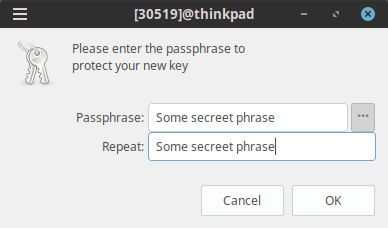
\includegraphics[scale=0.8]{res/3.pass1.png}
\end{center}

Был выбран слабый пароль для шифрования, о чём система меня предупредила. Продолжим с небезопасным паролем.
\begin{center}
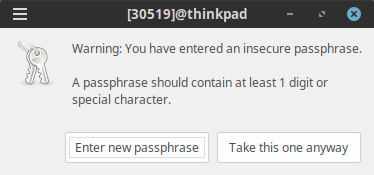
\includegraphics[scale=0.8]{res/3.pass2.png}
\end{center}

Текущий список ключей с keygrip (идемпотентный протокол хеширования для связи ключей)
\begin{Verbatim}[frame=single]
    smart@thinkpad$ gpg --list-keys --with-keygrip
    /home/smart/.gnupg/pubring.kbx
    ------------------------------
    pub   rsa4096 2023-02-11 [SC] [expires: 2023-03-04]
          9DAF94FCD9CA38BFD298BD0CA0B01E0BAB2AF7C6
          Keygrip = EC3AFAA6FD0AE71FB449D7D42849E173CF6CAAF4
    uid           [ultimate] Semen Martynov (Test digital sirnature) <martynov.sa@edu.spbstu.ru>
    sub   rsa4096 2023-02-11 [E] [expires: 2023-03-04]
          Keygrip = 16E5EFCBA47102BBA3A7C17D467D430C13D3D43E
\end{Verbatim}

\begin{itemize}
    \item \texttt{pub} -- публичный ключ (keygrip \texttt{EC3AFAA6FD0AE71FB449D7D42849E173CF6CAAF4});
    \item \texttt{uid} -- идентификатор (User-ID);
    \item \texttt{sub} -- публичный подключ (keygrip \texttt{16E5EFCBA47102BBA3A7C17D467D430C13D3D43E});
\end{itemize}

Список приватных ключей
\begin{Verbatim}[frame=single]
    smart@thinkpad$ gpg2 --list-secret-keys --with-keygrip
    /home/smart/.gnupg/pubring.kbx
    ------------------------------
    sec   rsa4096 2023-02-11 [SC] [expires: 2023-03-04]
        9DAF94FCD9CA38BFD298BD0CA0B01E0BAB2AF7C6
        Keygrip = EC3AFAA6FD0AE71FB449D7D42849E173CF6CAAF4
    uid           [ultimate] Semen Martynov (Test digital sirnature) <martynov.sa@edu.spbstu.ru>
    ssb   rsa4096 2023-02-11 [E] [expires: 2023-03-04]
        Keygrip = 16E5EFCBA47102BBA3A7C17D467D430C13D3D43E
\end{Verbatim}

\begin{itemize}
    \item \texttt{sec} -- секретный ключ (keygrip \texttt{EC3AFAA6FD0AE71FB449D7D42849E173CF6CAAF4});
    \item \texttt{uid} -- идентификатор (User-ID);
    \item \texttt{ssb} -- секретный подключ (keygrip \texttt{16E5EFCBA47102BBA3A7C17D467D430C13D3D43E});
\end{itemize}

Список подписей
\begin{Verbatim}[frame=single]
    smart@thinkpad$ gpg2 --list-signatures --with-keygrip
    /home/smart/.gnupg/pubring.kbx
    ------------------------------
    pub   rsa4096 2023-02-11 [SC] [expires: 2023-03-04]
        9DAF94FCD9CA38BFD298BD0CA0B01E0BAB2AF7C6
        Keygrip = EC3AFAA6FD0AE71FB449D7D42849E173CF6CAAF4
    uid           [ultimate] Semen Martynov (Test digital sirnature) <martynov.sa@edu.spbstu.ru>
    sig 3        A0B01E0BAB2AF7C6 2023-02-11  Semen Martynov (Test digital sirnature) <martynov.sa@edu.spbstu.ru>
    sub   rsa4096 2023-02-11 [E] [expires: 2023-03-04]
        Keygrip = 16E5EFCBA47102BBA3A7C17D467D430C13D3D43E
    sig          A0B01E0BAB2AF7C6 2023-02-11  Semen Martynov (Test digital sirnature) <martynov.sa@edu.spbstu.ru>
\end{Verbatim}

Отпечаток (fingerprint) подписи
\begin{Verbatim}[frame=single]
    smart@thinkpad$ gpg2 --fingerprint martynov.sa@edu.spbstu.ru
    pub   rsa4096 2023-02-11 [SC] [expires: 2023-03-04]
          9DAF 94FC D9CA 38BF D298  BD0C A0B0 1E0B AB2A F7C6
    uid           [ultimate] Semen Martynov (Test digital sirnature) <martynov.sa@edu.spbstu.ru>
    sub   rsa4096 2023-02-11 [E] [expires: 2023-03-04]
\end{Verbatim}

Исследуем содержимое директории \texttt{.gnupg}
\begin{Verbatim}[frame=single]
smart@thinkpad$ tree .gnupg/
.gnupg/
    openpgp-revocs.d
        9DAF94FCD9CA38BFD298BD0CA0B01E0BAB2AF7C6.rev
    private-keys-v1.d
        16E5EFCBA47102BBA3A7C17D467D430C13D3D43E.key
        EC3AFAA6FD0AE71FB449D7D42849E173CF6CAAF4.key
    pubring.kbx
    pubring.kbx~
    trustdb.gpg
\end{Verbatim}

В директории можно увидеть
\begin{itemize}
    \item \texttt{openpgp-revocs.d/9DAF94FCD9CA38BFD298BD0CA0B01E0BAB2AF7C6.rev} --  предварительно созданный сертификат отзыва. Имя файла соответствует отпечатку ключа. Всякий, у кого есть доступ к этому файлу, может отозвать соответствующий ключ.
    \item \texttt{private-keys-v1.d/EC3AFAA6FD0AE71FB449D7D42849E173CF6CAAF4.key} -- приватный ключ.
    \item \texttt{private-keys-v1.d/16E5EFCBA47102BBA3A7C17D467D430C13D3D43E.key} -- приватный подключ.
    \item \texttt{pubring.kbx} -- Таблица открытых ключей.
    \item \texttt{pubring.kbx~} -- Таблица открытых ключей (резервная копия).
    \item \texttt{trustdb.gpg} -- База данных доверия (Алиса подписала публичный ключ Боба, а Боб подписал публичный ключ Чарли; если Алиса получит публичный ключ Чарли, она сможет ему доверять, потому что ключ подписан тем, кому Алиса доверяет, т.е. Бобом).
\end{itemize}

\section*{3. Шифрование и подпись текста}
\addcontentsline{toc}{section}{3. Шифрование и подпись текста}
Для демонстрации возможностей утилиты, сгенерируем простой \texttt{Lorem Ipsum}.
\lstinputlisting[caption={Lorem Ipsum}, numbers=none]
{../Tasks/3_4_GnuPG_tool_utilisation/source_files/LoremIpsum.txt}

Теперь зашифруем файл с тестовым выводом
\begin{Verbatim}[frame=single]
    smart@thinkpad$ gpg2 \
     --armor \
     --recipient 9DAF94FCD9CA38BFD298BD0CA0B01E0BAB2AF7C6 \
     --encrypt LoremIpsum.txt
\end{Verbatim}

\lstinputlisting[caption={зашифрованный Lorem Ipsum}, numbers=none]
{../Tasks/3_4_GnuPG_tool_utilisation/source_files/LoremIpsum.txt.asc.nosign}

Далее расшифруем файл (операция потребует ввода приватной фразы!)
\begin{Verbatim}[frame=single]
    smart@thinkpad$ gpg2 \
     --recipient 9DAF94FCD9CA38BFD298BD0CA0B01E0BAB2AF7C6 \
     --decrypt LoremIpsum.txt.asc > LoremIpsum.decrypted.txt
\end{Verbatim}

Убедимся, что расшифрованный файл соответствует исходному.
\begin{Verbatim}[frame=single]
    smart@thinkpad$ shasum -a 1 LoremIpsum.txt LoremIpsum.decrypted.txt 
    014bbacd9d092d1f2272a3419125dbb2de0f3a6b  LoremIpsum.txt
    014bbacd9d092d1f2272a3419125dbb2de0f3a6b  LoremIpsum.decrypted.txt
\end{Verbatim}

\begin{Verbatim}[frame=single]
    smart@thinkpad$ gpg2 \
     --recipient 9DAF94FCD9CA38BFD298BD0CA0B01E0BAB2AF7C6 \
     --clearsign LoremIpsum.txt
\end{Verbatim}

\lstinputlisting[caption={Lorem Ipsum с цифровой подписью}, numbers=none]
{../Tasks/3_4_GnuPG_tool_utilisation/source_files/LoremIpsum.txt.asc}

Проверка цифровой подписи
\begin{Verbatim}[frame=single]
    smart@thinkpad$ gpg2 --verify LoremIpsum.txt.asc
    gpg: Signature made Sat 11 Feb 2023 07:57:52 PM MSK
    gpg:                using RSA key 9DAF94FCD9CA38BFD298BD0CA0B01E0BAB2AF7C6
    gpg: Good signature from "Semen Martynov (Test digital sirnature) <martynov.sa@edu.spbstu.ru>" [ultimate]
\end{Verbatim}

\section*{4. Прочие возможности использования GPG}
\addcontentsline{toc}{section}{4. Прочие возможности использования GPG}
Популярным способом использования GPG является цифровая подпись коммитов в git. Для этого в \texttt{.gitconfig} нужно добавить следующие параметры
\begin{Verbatim}[frame=single]
[commit]
        gpgsign = true
[user]
        signingkey = <KeyID>
[gpg]
        program = /bin/gpg
\end{Verbatim}

\section*{Выводы}
\addcontentsline{toc}{section}{Выводы}

В данной работе мы провели знакомство с возможностями утилиты GNU Privacy Guard. Разобрались с процессом генерации ключей и их хранением. Выполнили шифрование и сделали цифровую (присоединенную) подпись документа.

В практическом плане, использование GNU Privacy Guard позволяет подписывать коммитов в git для однозначного установления авторства.

\chapter*{Лабораторная работа 4. Импорт и экспорт ключей. Цифровая подпись}
\addcontentsline{toc}{chapter}{Лабораторная работа 4. Импорт и экспорт ключей. Цифровая подпись}

\textbf{Цель работы:} Знакомство с возможностями утилиты GNU Privacy Guard.

\section*{1. Экспорт открытого ключа}
\addcontentsline{toc}{section}{1. Экспорт открытого ключа}

Экспорт открытого ключа в текстовый файл
\begin{Verbatim}[frame=single]
    smart@thinkpad$ gpg2 \
     --armor \
     --export 9DAF94FCD9CA38BFD298BD0CA0B01E0BAB2AF7C6 > mykey.asc
\end{Verbatim}

\lstinputlisting[caption={Открытый ключ mykey.asc}, numbers=none]
{../Tasks/3_4_GnuPG_tool_utilisation/source_files/mykey.asc}

\section*{2. Создание электронной цифровой подписи (ЭЦП) файла}
\addcontentsline{toc}{section}{2. Создание электронной цифровой подписи (ЭЦП) файла}

Отсоединённая ЭЦП файла \texttt{mydocument.pdf} в текстовом формате (команда требует ввода ключевой фразы)
\begin{Verbatim}[frame=single]
    smart@thinkpad$ gpg2 \
     --sign \
     --detach-sign \
     --default-key 9DAF94FCD9CA38BFD298BD0CA0B01E0BAB2AF7C6 \
     --armor mydocument.pdf
\end{Verbatim}

\lstinputlisting[caption={Отсоединёння цифровая подпись для файла mydocument.pdf}, numbers=none]
{../Tasks/3_4_GnuPG_tool_utilisation/source_files/DigitalSignature/mydocument.pdf.asc}

Отсоединённая подпись в двоичном формате

\begin{Verbatim}[frame=single]
    smart@thinkpad$ gpg2 \
     --sign \
     --detach-sign \
     --default-key 9DAF94FCD9CA38BFD298BD0CA0B01E0BAB2AF7C6 \
     mydocument.pdf
\end{Verbatim}

Листинг двоичного файла не имеет смысла.

Встроенная в файл подпись в текстовом формате

\begin{Verbatim}[frame=single]
    smart@thinkpad$ gpg2 \
     --sign \
     --default-key 9DAF94FCD9CA38BFD298BD0CA0B01E0BAB2AF7C6 \
     --armor mydocument.pdf
\end{Verbatim}

Листинг не имеет смысла, т.к. включает объёмный исходный PDF-файл.

Встроенная в файл подпись в двоичном формате

\begin{Verbatim}[frame=single]
    smart@thinkpad$ gpg2 \
     --sign \
     --default-key 9DAF94FCD9CA38BFD298BD0CA0B01E0BAB2AF7C6 \
     mydocument.pdf
\end{Verbatim}

Листинг не имеет смысла, т.к. сгенерирован бинарный файл.

\section*{3. Импорт открытого ключа}
\addcontentsline{toc}{section}{3. Импорт открытого ключа}

Возьмём файл цифровой подписи GnuPG проекта файлового шифровальщика VeraCrypt.

\begin{Verbatim}[frame=single]
    smart@thinkpad$ wget https://www.idrix.fr/VeraCrypt/VeraCrypt_PGP_public_key.asc
\end{Verbatim}

Перед импортом, можно удостовериться, что цифровая подпись содержит правильный ID.
\begin{Verbatim}[frame=single]
    smart@thinkpad$ gpg --show-keys VeraCrypt_PGP_public_key.asc
    pub   rsa4096 2018-09-11 [SC]
        5069A233D55A0EEB174A5FC3821ACD02680D16DE
    uid                      VeraCrypt Team (2018 - Supersedes Key ID=0x54DDD393) <veracrypt@idrix.fr>
    sub   rsa4096 2018-09-11 [E]
    sub   rsa4096 2018-09-11 [A]
\end{Verbatim}

После этого можно импортировать файл
\begin{Verbatim}[frame=single]
    smart@thinkpad$ gpg --import VeraCrypt_PGP_public_key.asc 
    gpg: key 821ACD02680D16DE: 1 signature not checked due to a missing key
    gpg: key 821ACD02680D16DE: public key "VeraCrypt Team (2018 - Supersedes Key ID=0x54DDD393) <veracrypt@idrix.fr>" imported
    gpg: Total number processed: 1
    gpg:               imported: 1
    gpg: marginals needed: 3  completes needed: 1  trust model: pgp
    gpg: depth: 0  valid:   1  signed:   0  trust: 0-, 0q, 0n, 0m, 0f, 1u
    gpg: next trustdb check due at 2023-03-04
\end{Verbatim}

Для проверки подписи \underline{не обязательно} устанавливать доверительные отношения с импортированным ключом.

\section*{4. Проверка ЭЦП}
\addcontentsline{toc}{section}{4. Проверка ЭЦП}

Для проверки, возьмём архив с исходными кодами и отсоединённую подпись в двоичном формате
\begin{Verbatim}[frame=single]
    smart@thinkpad$ wget https://launchpad.net/veracrypt/trunk/1.25.9/+download/VeraCrypt_1.25.9_Source.tar.bz2
    smart@thinkpad$ wget https://launchpad.net/veracrypt/trunk/1.25.9/+download/VeraCrypt_1.25.9_Source.tar.bz2.sig
\end{Verbatim}

Теперь всё готово для проверки.
\begin{Verbatim}[frame=single]
    smart@thinkpad$ gpg --verify VeraCrypt_1.25.9_Source.tar.bz2.sig VeraCrypt_1.25.9_Source.tar.bz2
    gpg: Signature made Sun 20 Feb 2022 04:18:32 PM MSK
    gpg:                using RSA key 5069A233D55A0EEB174A5FC3821ACD02680D16DE
    gpg: Good signature from "VeraCrypt Team (2018 - Supersedes Key ID=0x54DDD393) <veracrypt@idrix.fr>" [unknown]
    gpg: WARNING: This key is not certified with a trusted signature!
    gpg:          There is no indication that the signature belongs to the owner.
    Primary key fingerprint: 5069 A233 D55A 0EEB 174A  5FC3 821A CD02 680D 16DE
\end{Verbatim}

Ожидаемый результат -- \texttt{Good signature}.

Остальные предупреждения, связанные с отсутствием доверия, можно игнорировать.

\section*{5. Экспорт/импорт на ключевые сервера}
\addcontentsline{toc}{section}{5. Экспорт/импорт на ключевые сервера}

Экспорт своего ключа
\begin{Verbatim}[frame=single]
    smart@thinkpad$ gpg --keyserver hkp://keyserver.ubuntu.com --send-key 9DAF94FCD9CA38BFD298BD0CA0B01E0BAB2AF7C6
    gpg: sending key A0B01E0BAB2AF7C6 to hkp://keyserver.ubuntu.com
\end{Verbatim}

Теперь воспользуемся поиском, для обнаружения этого ключа на удалённом сервере
\begin{Verbatim}[frame=single]
    smart@thinkpad$ gpg --keyserver hkp://keyserver.ubuntu.com --search-keys martynov.sa@edu.spbstu.ru
    gpg: data source: http://162.213.33.9:11371
    (1)	Semen Martynov (Test digital sirnature) <martynov.sa@edu.spbstu.ru>
    	  4096 bit RSA key A0B01E0BAB2AF7C6, created: 2023-02-11
    Keys 1-1 of 1 for "martynov.sa@edu.spbstu.ru".  Enter number(s), N)ext, or Q)uit >

    smart@thinkpad$ gpg --keyserver hkp://keyserver.ubuntu.com --list-sigs martynov.sa@edu.spbstu.ru
    pub   rsa4096 2023-02-11 [SC] [expires: 2023-03-04]
          9DAF94FCD9CA38BFD298BD0CA0B01E0BAB2AF7C6
    uid           [ultimate] Semen Martynov (Test digital sirnature) <martynov.sa@edu.spbstu.ru>
    sig 3        A0B01E0BAB2AF7C6 2023-02-11  Semen Martynov (Test digital sirnature) <martynov.sa@edu.spbstu.ru>
    sub   rsa4096 2023-02-11 [E] [expires: 2023-03-04]
    sig          A0B01E0BAB2AF7C6 2023-02-11  Semen Martynov (Test digital sirnature) <martynov.sa@edu.spbstu.ru>
\end{Verbatim}

Так же легко можно импортировать ключи с удалённого сервера
\begin{Verbatim}[frame=single]
    smart@thinkpad$ gpg --keyserver pgp.mit.edu --recv-keys DAD95197
    gpg: key FBF1FC87DAD95197: public key "Ashish Aniyan <aaniyan@verimatrix.com>" imported
    gpg: Total number processed: 1
    gpg:               imported: 1
\end{Verbatim}

Для интеграции GPG заработал в почтовом клиенте \texttt{Mutt}, нужно в конфигурационный файл \texttt{~/.muttrc дописать}
\begin{Verbatim}[frame=single]
    set crypt_use_gpgme=yes
    set crypt_autosign=yes
    set crypt_replyencrypt=yes
\end{Verbatim}

\section*{Выводы}
\addcontentsline{toc}{section}{Выводы}

В данной работе мы сравнили различные виды электронных цифровых подписей:
\begin{itemize}
    \item Отсоединённую ЭЦП в текстовом формате
    \item Отсоединённую ЭЦП в бинарном формате
    \item Присоединенную ЭЦП в текстовом формате
    \item Присоединенную ЭЦП в бинарном формате
\end{itemize}

Работа с отсоединённой подписью удобнее. В цифровом виде подпись занимает меньше места.

В практическом плане, использование GNU Privacy Guard позволяет верифицировать не только документы, но и цифровые пакеты при распространении через Интернет.

\chapter*{Лабораторная работа 5. Анализатор сетевого трафика Wireshark}
\addcontentsline{toc}{chapter}{Лабораторная работа 5. Анализатор сетевого трафика Wireshark}

\textbf{Цель работы:} Знакомство с возможностями анализатора сетевого трафика Wireshark.

\section*{1. Установка}
\addcontentsline{toc}{section}{1. Установка}

Для использования \texttt{wireshark} в графическом режиме, потребуется пакет \texttt{wireshark-qt}.
\begin{Verbatim}[frame=single,breaklines=true,breakanywhere=true]
    smart@thinkpad$ sudo pacman -S wireshark-qt
    resolving dependencies...
    looking for conflicting packages...

    Packages (10) bcg729-1.1.1-1  c-ares-1.19.0-1  cdparanoia-10.2-8
                gst-plugins-base-1.22.0-3  libmaxminddb-1.7.1-1
                qt5-multimedia-5.15.8+kde+r2-1  sbc-2.0-1  spandsp-0.0.6-4
                wireshark-cli-4.0.3-1  wireshark-qt-4.0.3-1

    Total Download Size:    28.58 MiB
    Total Installed Size:  138.16 MiB

    :: Proceed with installation? [Y/n] 
    :: Retrieving packages...
    spandsp-0.0.6-4-...   424.1 KiB  1820 KiB/s 00:00 [######################] 100%
    qt5-multimedia-5...   763.0 KiB  2.79 MiB/s 00:00 [######################] 100%
    c-ares-1.19.0-1-...   205.7 KiB  5.02 MiB/s 00:00 [######################] 100%
    sbc-2.0-1-x86_64       47.9 KiB  1197 KiB/s 00:00 [######################] 100%
    bcg729-1.1.1-1-x...    37.6 KiB   939 KiB/s 00:00 [######################] 100%
    libmaxminddb-1.7...    23.9 KiB  1193 KiB/s 00:00 [######################] 100%
    gst-plugins-base...   316.3 KiB   703 KiB/s 00:00 [######################] 100%
    wireshark-qt-4.0...     4.1 MiB  2.56 MiB/s 00:02 [######################] 100%
    wireshark-cli-4.0.3-1-x86_64                                                                                       22.7 MiB  3.37 MiB/s 00:07 [########################################################################################] 100%
    Total (9/9)                                                                                                        28.6 MiB  4.21 MiB/s 00:07 [########################################################################################] 100%
    (10/10) checking keys in keyring                                                                                                               [########################################################################################] 100%
    (10/10) checking package integrity                                                                                                             [########################################################################################] 100%
    (10/10) loading package files                                                                                                                  [########################################################################################] 100%
    (10/10) checking for file conflicts                                                                                                            [########################################################################################] 100%
    (10/10) checking available disk space                                                                                                          [########################################################################################] 100%
    :: Processing package changes...
    ( 1/10) installing cdparanoia                                                                                                                  [########################################################################################] 100%
    ( 2/10) installing gst-plugins-base                                                                                                            [########################################################################################] 100%
    ( 3/10) installing qt5-multimedia                                                                                                              [########################################################################################] 100%
    Optional dependencies for qt5-multimedia
        qt5-declarative: QML bindings [installed]
        gst-plugins-good: camera support, additional plugins
        gst-plugins-bad: camera support, additional plugins
        gst-plugins-ugly: additional plugins
        gst-libav: ffmpeg plugin
    ( 4/10) installing c-ares                                                                                                                      [########################################################################################] 100%
    ( 5/10) installing libmaxminddb                                                                                                                [########################################################################################] 100%
    Optional dependencies for libmaxminddb
        geoip2-database: IP geolocation databases
    ( 6/10) installing spandsp                                                                                                                     [########################################################################################] 100%
    ( 7/10) installing sbc                                                                                                                         [########################################################################################] 100%
    ( 8/10) installing bcg729                                                                                                                      [########################################################################################] 100%
    ( 9/10) installing wireshark-cli                                                                                                               [########################################################################################] 100%
    NOTE: To run wireshark as normal user you have to add yourself into wireshark group
    (10/10) installing wireshark-qt                                                                                                                [########################################################################################] 100%
    :: Running post-transaction hooks...
    (1/5) Creating system user accounts...
    Creating group 'wireshark' with GID 150.
    (2/5) Arming ConditionNeedsUpdate...
    (3/5) Updating the MIME type database...
    (4/5) Updating icon theme caches...
    (5/5) Updating the desktop file MIME type cache...
\end{Verbatim}

\section*{2. Анализ ICMP трафика}
\addcontentsline{toc}{section}{2. Анализ ICMP трафика}

Генерация трафика:
Для использования \texttt{wireshark} в графическом режиме, потребуется пакет \texttt{wireshark-qt}.
\begin{Verbatim}[frame=single,breaklines=true,breakanywhere=true]
    smart@thinkpad$ ping 192.168.124.1
\end{Verbatim}

Фильтрация \texttt{ICMP} пакетов в \texttt{wireshark}
\begin{center}
    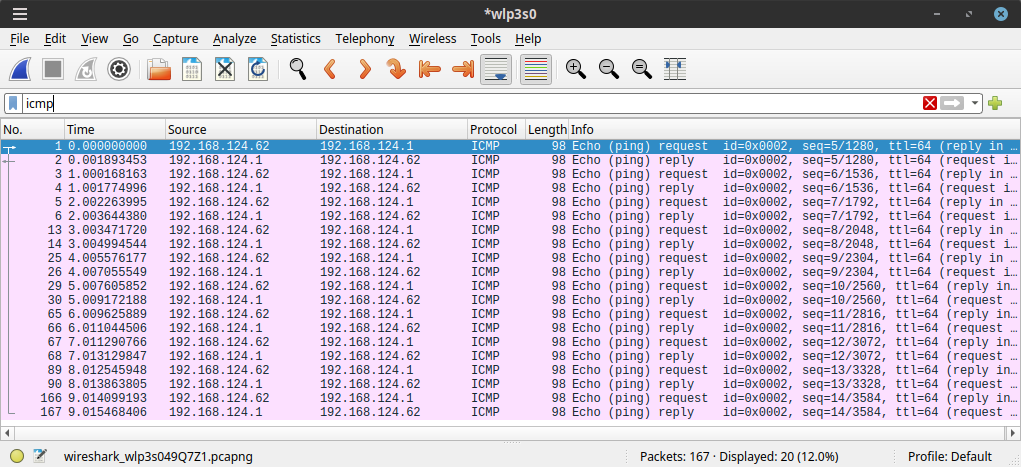
\includegraphics[scale=0.6]{res/5.wireshark-icmp.png}
\end{center}

Рассмотрим \texttt{ICMP} пакет, полученный в качестве эхо-ответа от удалённого хоста.

\subsection*{Канальный уровень (data link): Ethernet фрейм}
\addcontentsline{toc}{subsection}{Канальный уровень (data link): Ethernet фрейм}

Первые 6 байт -- MAC-адрес получателя пакета (\texttt{14:5a:fc:0d:56:2d}).

\fbox{
    \parbox{\textwidth}{%
    \texttt{\noindent
0000|   \hl{14 5a fc 0d 56 2d} 34 ce 00 37 d9 03 08 00 45 00\\
0010|   00 54 20 30 00 00 40 01 e0 e8 c0 a8 7c 01 c0 a8\\
0020|   7c 3e 00 00 d3 bd 00 02 00 0e 7a c1 e8 63 00 00\\
0030|   00 00 08 3a 02 00 00 00 00 00 10 11 12 13 14 15\\
0040|   16 17 18 19 1a 1b 1c 1d 1e 1f 20 21 22 23 24 25\\
0050|   26 27 28 29 2a 2b 2c 2d 2e 2f 30 31 32 33 34 35\\
0060|   36 37
    }}%
}

Следующие 6 байт -- MAC-адрес отправителя пакета (\texttt{34:ce:00:37:d9:03}).

\fbox{
    \parbox{\textwidth}{%
    \texttt{\noindent
0000|   14 5a fc 0d 56 2d \hl{34 ce 00 37 d9 03} 08 00 45 00\\
0010|   00 54 20 30 00 00 40 01 e0 e8 c0 a8 7c 01 c0 a8\\
0020|   7c 3e 00 00 d3 bd 00 02 00 0e 7a c1 e8 63 00 00\\
0030|   00 00 08 3a 02 00 00 00 00 00 10 11 12 13 14 15\\
0040|   16 17 18 19 1a 1b 1c 1d 1e 1f 20 21 22 23 24 25\\
0050|   26 27 28 29 2a 2b 2c 2d 2e 2f 30 31 32 33 34 35\\
0060|   36 37
    }}%
}

Тип пакетов -- IPv4 (\texttt{0x0800}). Полный список типов в удобном виде можно посмотреть в Wikipedia:\\\url{https://en.wikipedia.org/wiki/EtherType}

\fbox{
    \parbox{\textwidth}{%
    \texttt{\noindent
0000|   14 5a fc 0d 56 2d 34 ce 00 37 d9 03 \hl{08 00} 45 00\\
0010|   00 54 20 30 00 00 40 01 e0 e8 c0 a8 7c 01 c0 a8\\
0020|   7c 3e 00 00 d3 bd 00 02 00 0e 7a c1 e8 63 00 00\\
0030|   00 00 08 3a 02 00 00 00 00 00 10 11 12 13 14 15\\
0040|   16 17 18 19 1a 1b 1c 1d 1e 1f 20 21 22 23 24 25\\
0050|   26 27 28 29 2a 2b 2c 2d 2e 2f 30 31 32 33 34 35\\
0060|   36 37
    }}%
}

\subsection*{Сетевой уровень (network): IP пакет}
\addcontentsline{toc}{subsection}{Сетевой уровень (network): IP пакет}

Первые 4 бита указывают на версию IP. Код \texttt{0100} указывает на 4-ю версию. Структуру IPv4 пакета можно посмотреть в Wikipedia:\\\url{https://en.wikipedia.org/wiki/Internet_Protocol_version_4}

Следующие 4 бита передают длину хедера пакета. Код \texttt{0101} соответствует длинне в 20 байт.

\texttt{wireshark} показывает байт целиком.

\fbox{
    \parbox{\textwidth}{%
    \texttt{\noindent
0000|   14 5a fc 0d 56 2d 34 ce 00 37 d9 03 08 00 \hl{45} 00\\
0010|   00 54 20 30 00 00 40 01 e0 e8 c0 a8 7c 01 c0 a8\\
0020|   7c 3e 00 00 d3 bd 00 02 00 0e 7a c1 e8 63 00 00\\
0030|   00 00 08 3a 02 00 00 00 00 00 10 11 12 13 14 15\\
0040|   16 17 18 19 1a 1b 1c 1d 1e 1f 20 21 22 23 24 25\\
0050|   26 27 28 29 2a 2b 2c 2d 2e 2f 30 31 32 33 34 35\\
0060|   36 37
    }}%
}

Дальше идут сервисные поля \texttt{DSCP} (разделения трафика на классы обслуживания) и \texttt{ECN} (предупреждение о перегрузке сети без потери пакетов), в суть которых мы не будем углубляться, т.к. они всё равно не используются в данном случа.

\fbox{
    \parbox{\textwidth}{%
    \texttt{\noindent
0000|   14 5a fc 0d 56 2d 34 ce 00 37 d9 03 08 00 45 \hl{00}\\
0010|   00 54 20 30 00 00 40 01 e0 e8 c0 a8 7c 01 c0 a8\\
0020|   7c 3e 00 00 d3 bd 00 02 00 0e 7a c1 e8 63 00 00\\
0030|   00 00 08 3a 02 00 00 00 00 00 10 11 12 13 14 15\\
0040|   16 17 18 19 1a 1b 1c 1d 1e 1f 20 21 22 23 24 25\\
0050|   26 27 28 29 2a 2b 2c 2d 2e 2f 30 31 32 33 34 35\\
0060|   36 37
    }}%
}

Следующие 16 бит это полный размер пакета в байтах, включая заголовок и данные. По RFC, он может быть от 20 до 65535 байт. А нашем случае -- 84.

\fbox{
    \parbox{\textwidth}{%
    \texttt{\noindent
0000|   14 5a fc 0d 56 2d 34 ce 00 37 d9 03 08 00 45 00\\
0010|   \hl{00 54} 20 30 00 00 40 01 e0 e8 c0 a8 7c 01 c0 a8\\
0020|   7c 3e 00 00 d3 bd 00 02 00 0e 7a c1 e8 63 00 00\\
0030|   00 00 08 3a 02 00 00 00 00 00 10 11 12 13 14 15\\
0040|   16 17 18 19 1a 1b 1c 1d 1e 1f 20 21 22 23 24 25\\
0050|   26 27 28 29 2a 2b 2c 2d 2e 2f 30 31 32 33 34 35\\
0060|   36 37
    }}%
}

Далее идёт уникальный идентификатор, используемый для идентификации фрагментов пакета, если он был фрагментирован.

\fbox{
    \parbox{\textwidth}{%
    \texttt{\noindent
0000|   14 5a fc 0d 56 2d 34 ce 00 37 d9 03 08 00 45 00\\
0010|   00 54 \hl{20 30} 00 00 40 01 e0 e8 c0 a8 7c 01 c0 a8\\
0020|   7c 3e 00 00 d3 bd 00 02 00 0e 7a c1 e8 63 00 00\\
0030|   00 00 08 3a 02 00 00 00 00 00 10 11 12 13 14 15\\
0040|   16 17 18 19 1a 1b 1c 1d 1e 1f 20 21 22 23 24 25\\
0050|   26 27 28 29 2a 2b 2c 2d 2e 2f 30 31 32 33 34 35\\
0060|   36 37
    }}%
}

Следующие три бита -- поле флагов. Биты, от старшего к младшему, означают:
\begin{itemize}
    \item 0: Зарезервирован, должен быть равен 0
    \item 1: Не фрагментировать
    \item 2: У пакета ещё есть фрагменты
\end{itemize}

И после этого ещё 13 бит для указания смещение поля данных текущего фрагмента относительно начала поля данных первого фрагментированного пакета в блоках по 8 байт.

\fbox{
    \parbox{\textwidth}{%
    \texttt{\noindent
0000|   14 5a fc 0d 56 2d 34 ce 00 37 d9 03 08 00 45 00\\
0010|   00 54 20 30 \hl{00 00} 40 01 e0 e8 c0 a8 7c 01 c0 a8\\
0020|   7c 3e 00 00 d3 bd 00 02 00 0e 7a c1 e8 63 00 00\\
0030|   00 00 08 3a 02 00 00 00 00 00 10 11 12 13 14 15\\
0040|   16 17 18 19 1a 1b 1c 1d 1e 1f 20 21 22 23 24 25\\
0050|   26 27 28 29 2a 2b 2c 2d 2e 2f 30 31 32 33 34 35\\
0060|   36 37
    }}%
}

Время жизни пакета (Time to Live) задаёт максимальное количество маршрутизаторов (хопов) на пути следования пакета. Максимальное значение TTL=255, но чаще встречается TTL=64.

\fbox{
    \parbox{\textwidth}{%
    \texttt{\noindent
0000|   14 5a fc 0d 56 2d 34 ce 00 37 d9 03 08 00 45 00\\
0010|   00 54 20 30 00 00 \hl{40} 01 e0 e8 c0 a8 7c 01 c0 a8\\
0020|   7c 3e 00 00 d3 bd 00 02 00 0e 7a c1 e8 63 00 00\\
0030|   00 00 08 3a 02 00 00 00 00 00 10 11 12 13 14 15\\
0040|   16 17 18 19 1a 1b 1c 1d 1e 1f 20 21 22 23 24 25\\
0050|   26 27 28 29 2a 2b 2c 2d 2e 2f 30 31 32 33 34 35\\
0060|   36 37
    }}%
}

Следующее поле показывает, данные какого протокола IP содержит пакет (к примеру, это может быть TCP). Список кодов можно посмотреть на сайте IANA:\\\url{https://www.iana.org/assignments/protocol-numbers/protocol-numbers.xml}

Код \texttt{01} соответствует ICMP.

\fbox{
    \parbox{\textwidth}{%
    \texttt{\noindent
0000|   14 5a fc 0d 56 2d 34 ce 00 37 d9 03 08 00 45 00\\
0010|   00 54 20 30 00 00 40 \hl{01} e0 e8 c0 a8 7c 01 c0 a8\\
0020|   7c 3e 00 00 d3 bd 00 02 00 0e 7a c1 e8 63 00 00\\
0030|   00 00 08 3a 02 00 00 00 00 00 10 11 12 13 14 15\\
0040|   16 17 18 19 1a 1b 1c 1d 1e 1f 20 21 22 23 24 25\\
0050|   26 27 28 29 2a 2b 2c 2d 2e 2f 30 31 32 33 34 35\\
0060|   36 37
    }}%
}

Контрольная сумма заголовка занимает следующие 2-байта и используемая для проверки целостности заголовка

\fbox{
    \parbox{\textwidth}{%
    \texttt{\noindent
0000|   14 5a fc 0d 56 2d 34 ce 00 37 d9 03 08 00 45 00\\
0010|   00 54 20 30 00 00 40 01 \hl{e0 e8} c0 a8 7c 01 c0 a8\\
0020|   7c 3e 00 00 d3 bd 00 02 00 0e 7a c1 e8 63 00 00\\
0030|   00 00 08 3a 02 00 00 00 00 00 10 11 12 13 14 15\\
0040|   16 17 18 19 1a 1b 1c 1d 1e 1f 20 21 22 23 24 25\\
0050|   26 27 28 29 2a 2b 2c 2d 2e 2f 30 31 32 33 34 35\\
0060|   36 37
    }}%
}

Далее 32-битный адрес отправителя пакета (Может не совпадать с настоящим адресом отправителя из-за трансляции адресов -- NAT)

\fbox{
    \parbox{\textwidth}{%
    \texttt{\noindent
0000|   14 5a fc 0d 56 2d 34 ce 00 37 d9 03 08 00 45 00\\
0010|   00 54 20 30 00 00 40 01 e0 e8 \hl{c0 a8 7c 01} c0 a8\\
0020|   7c 3e 00 00 d3 bd 00 02 00 0e 7a c1 e8 63 00 00\\
0030|   00 00 08 3a 02 00 00 00 00 00 10 11 12 13 14 15\\
0040|   16 17 18 19 1a 1b 1c 1d 1e 1f 20 21 22 23 24 25\\
0050|   26 27 28 29 2a 2b 2c 2d 2e 2f 30 31 32 33 34 35\\
0060|   36 37
    }}%
}

И 32-битный адрес получателя пакета (учитывая, что это \texttt{ICMP}-ответ, получателем будет хост, на котором запущен \texttt{ping}).

\fbox{
    \parbox{\textwidth}{%
    \texttt{\noindent
0000|   14 5a fc 0d 56 2d 34 ce 00 37 d9 03 08 00 45 00\\
0010|   00 54 20 30 00 00 40 01 e0 e8 c0 a8 7c 01 \hl{c0 a8}\\
0020|   \hl{7c 3e} 00 00 d3 bd 00 02 00 0e 7a c1 e8 63 00 00\\
0030|   00 00 08 3a 02 00 00 00 00 00 10 11 12 13 14 15\\
0040|   16 17 18 19 1a 1b 1c 1d 1e 1f 20 21 22 23 24 25\\
0050|   26 27 28 29 2a 2b 2c 2d 2e 2f 30 31 32 33 34 35\\
0060|   36 37
    }}%
}

\subsection*{Сетевой уровень (network): ICMP пакет}
\addcontentsline{toc}{subsection}{Сетевой уровень (network): ICMP пакет}

Первый байт указывает на тип пакета.

Код \texttt{0} соответствует \texttt{ICMP}-ответу. Список кодов и заголовков можно посмотреть в Wikipedia:\\\url{https://en.wikipedia.org/wiki/Internet_Control_Message_Protocol}

\fbox{
    \parbox{\textwidth}{%
    \texttt{\noindent
0000|   14 5a fc 0d 56 2d 34 ce 00 37 d9 03 08 00 45 00\\
0010|   00 54 20 30 00 00 40 01 e0 e8 c0 a8 7c 01 c0 a8\\
0020|   7c 3e \hl{00} 00 d3 bd 00 02 00 0e 7a c1 e8 63 00 00\\
0030|   00 00 08 3a 02 00 00 00 00 00 10 11 12 13 14 15\\
0040|   16 17 18 19 1a 1b 1c 1d 1e 1f 20 21 22 23 24 25\\
0050|   26 27 28 29 2a 2b 2c 2d 2e 2f 30 31 32 33 34 35\\
0060|   36 37
    }}%
}

Следующий байт -- код, который зависит от типа пакета. Для \texttt{ICMP}-ответа возможно только 0-е значение.

\fbox{
    \parbox{\textwidth}{%
    \texttt{\noindent
0000|   14 5a fc 0d 56 2d 34 ce 00 37 d9 03 08 00 45 00\\
0010|   00 54 20 30 00 00 40 01 e0 e8 c0 a8 7c 01 c0 a8\\
0020|   7c 3e 00 \hl{00} d3 bd 00 02 00 0e 7a c1 e8 63 00 00\\
0030|   00 00 08 3a 02 00 00 00 00 00 10 11 12 13 14 15\\
0040|   16 17 18 19 1a 1b 1c 1d 1e 1f 20 21 22 23 24 25\\
0050|   26 27 28 29 2a 2b 2c 2d 2e 2f 30 31 32 33 34 35\\
0060|   36 37
    }}%
}

Ещё два байта нужны для передачи контрльной суммы.

\fbox{
    \parbox{\textwidth}{%
    \texttt{\noindent
0000|   14 5a fc 0d 56 2d 34 ce 00 37 d9 03 08 00 45 00\\
0010|   00 54 20 30 00 00 40 01 e0 e8 c0 a8 7c 01 c0 a8\\
0020|   7c 3e 00 00 \hl{d3 bd} 00 02 00 0e 7a c1 e8 63 00 00\\
0030|   00 00 08 3a 02 00 00 00 00 00 10 11 12 13 14 15\\
0040|   16 17 18 19 1a 1b 1c 1d 1e 1f 20 21 22 23 24 25\\
0050|   26 27 28 29 2a 2b 2c 2d 2e 2f 30 31 32 33 34 35\\
0060|   36 37
    }}%
}

Следующие 4 байта так же зависят от типа и кода.

\fbox{
    \parbox{\textwidth}{%
    \texttt{\noindent
0000|   14 5a fc 0d 56 2d 34 ce 00 37 d9 03 08 00 45 00\\
0010|   00 54 20 30 00 00 40 01 e0 e8 c0 a8 7c 01 c0 a8\\
0020|   7c 3e 00 00 d3 bd \hl{00 02 00 0e} 7a c1 e8 63 00 00\\
0030|   00 00 08 3a 02 00 00 00 00 00 10 11 12 13 14 15\\
0040|   16 17 18 19 1a 1b 1c 1d 1e 1f 20 21 22 23 24 25\\
0050|   26 27 28 29 2a 2b 2c 2d 2e 2f 30 31 32 33 34 35\\
0060|   36 37
    }}%
}

Далее идёт временная метка, для расчёта задержки при доставке сообщения

\fbox{
    \parbox{\textwidth}{%
    \texttt{\noindent
0000|   14 5a fc 0d 56 2d 34 ce 00 37 d9 03 08 00 45 00\\
0010|   00 54 20 30 00 00 40 01 e0 e8 c0 a8 7c 01 c0 a8\\
0020|   7c 3e 00 00 d3 bd 00 02 00 0e \hl{7a c1 e8 63 00 00}\\
0030|   \hl{00 00} 08 3a 02 00 00 00 00 00 10 11 12 13 14 15\\
0040|   16 17 18 19 1a 1b 1c 1d 1e 1f 20 21 22 23 24 25\\
0050|   26 27 28 29 2a 2b 2c 2d 2e 2f 30 31 32 33 34 35\\
0060|   36 37
    }}%
}

Оставшиеся 48 байт присылают в содержат тело запроса, полученное \texttt{ICMP}-сервером (по этой причине схема и получила название "эхо").

\fbox{
    \parbox{\textwidth}{%
    \texttt{\noindent
0000|   14 5a fc 0d 56 2d 34 ce 00 37 d9 03 08 00 45 00\\
0010|   00 54 20 30 00 00 40 01 e0 e8 c0 a8 7c 01 c0 a8\\
0020|   7c 3e 00 00 d3 bd 00 02 00 0e 7a c1 e8 63 00 00\\
0030|   00 00 \hl{08 3a 02 00 00 00 00 00 10 11 12 13 14 15}\\
0040|   \hl{16 17 18 19 1a 1b 1c 1d 1e 1f 20 21 22 23 24 25}\\
0050|   \hl{26 27 28 29 2a 2b 2c 2d 2e 2f 30 31 32 33 34 35}\\
0060|   \hl{36 37}
    }}%
}

Значения для полей при различных режимах работы \texttt{ICMP} приведены в Wikipedia:\\\url{https://en.wikipedia.org/wiki/Internet_Control_Message_Protocol}

\section*{3. Анализ ARP трафика}
\addcontentsline{toc}{section}{3. Анализ ARP трафика}

Протокол разрешения адресов (\texttt{Address Resolution Protocol}, \texttt{ARP}) используется в компьютерных сетях для сопоставления \texttt{IP}-адресов и \texttt{MAC}-адресов в рамках одного широковещательного домена. Механизм сопоставления называют "\texttt{ARP}-таблицами" и этот механизм подвержен различными атакам (типа переполнения размерности) для встраивания в цепочку передачи (\texttt{Man-in-the-middle}).

Отображение \texttt{ARP}-таблицы на беспроводном интерфейсе
\begin{Verbatim}[frame=single,breaklines=true,breakanywhere=true]
    smart@thinkpad$ ip neigh show dev wlp3s0
    192.168.124.1 lladdr 34:ce:00:37:d9:03 REACHABLE 
    fe80::36ce:ff:fe37:d903 lladdr 34:ce:00:37:d9:03 router REACHABLE 
\end{Verbatim}

Фильтрация \texttt{ARP} пакетов в \texttt{wireshark}
\begin{center}
    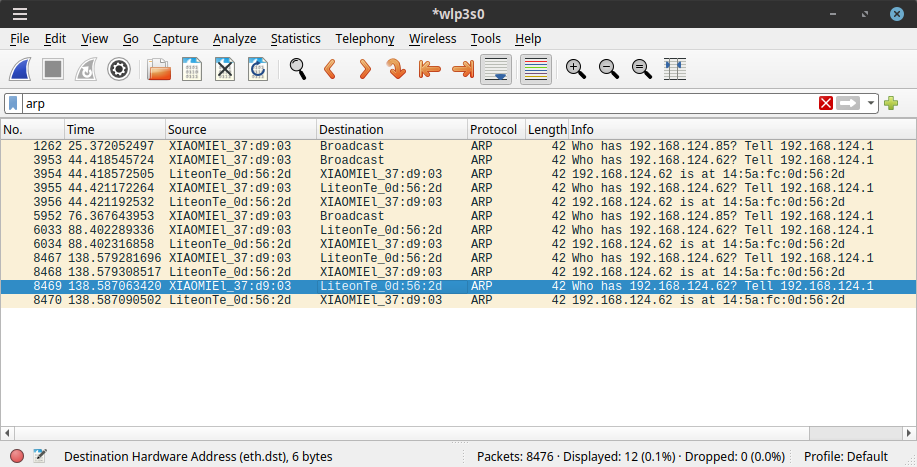
\includegraphics[scale=0.6]{res/5.wireshark-arp.png}
\end{center}

\subsection*{Канальный уровень (data link): Ethernet фрейм}
\addcontentsline{toc}{subsection}{Канальный уровень (data link): Ethernet фрейм}

\texttt{MAC}-адрес получателя \texttt{ff:ff:ff:ff:ff:ff}. Широковещательное (Broadcast) сообщение.

\fbox{
    \parbox{\textwidth}{%
    \texttt{\noindent
0000|   \hl{ff ff ff ff ff ff} 34 ce 00 37 d9 03 08 06 00 01\\
0010|   08 00 06 04 00 01 34 ce 00 37 d9 03 c0 a8 7c 01\\
0020|   00 00 00 00 00 00 c0 a8 7c 55
    }}%
}

\texttt{MAC}-адрес отправителя \texttt{34:ce:00:37:d9:03}

\fbox{
    \parbox{\textwidth}{%
    \texttt{\noindent
0000|   ff ff ff ff ff ff \hl{34 ce 00 37 d9 03} 08 06 00 01\\
0010|   08 00 06 04 00 01 34 ce 00 37 d9 03 c0 a8 7c 01\\
0020|   00 00 00 00 00 00 c0 a8 7c 55
    }}%
}

Тип сообщения -- \texttt{ARP} (\texttt{0x0806}). Справочник в Wikipedia:\\\url{https://en.wikipedia.org/wiki/EtherType}

\fbox{
    \parbox{\textwidth}{%
    \texttt{\noindent
0000|   ff ff ff ff ff ff 34 ce 00 37 d9 03 \hl{08 06} 00 01\\
0010|   08 00 06 04 00 01 34 ce 00 37 d9 03 c0 a8 7c 01\\
0020|   00 00 00 00 00 00 c0 a8 7c 55
    }}%
}

\subsection*{Сетевой уровень (network): ARP пакет}
\addcontentsline{toc}{subsection}{Сетевой уровень (network): ARP пакет}

Структура пакетов и значения флагов описаны в Wikipedia:\\\url{https://ru.wikipedia.org/wiki/ARP}

Первые два байта -- тип канального протокола. \texttt{Ethernet} имеет номер \texttt{0x0001}.

\fbox{
    \parbox{\textwidth}{%
    \texttt{\noindent
0000|   ff ff ff ff ff ff 34 ce 00 37 d9 03 08 06 \hl{00 01}\\
0010|   08 00 06 04 00 01 34 ce 00 37 d9 03 c0 a8 7c 01\\
0020|   00 00 00 00 00 00 c0 a8 7c 55
    }}%
}

Ещё два байта для кода сетевого протокола. Для \texttt{IPv4} код \texttt{0x0800}.

\fbox{
    \parbox{\textwidth}{%
    \texttt{\noindent
0000|   ff ff ff ff ff ff 34 ce 00 37 d9 03 08 06 00 01\\
0010|   \hl{08 00} 06 04 00 01 34 ce 00 37 d9 03 c0 a8 7c 01\\
0020|   00 00 00 00 00 00 c0 a8 7c 55
    }}%
}

Длина физического адреса в байтах. Адреса \texttt{Ethernet} имеют длину 6 байт (\texttt{0x06})

\fbox{
    \parbox{\textwidth}{%
    \texttt{\noindent
0000|   ff ff ff ff ff ff 34 ce 00 37 d9 03 08 06 00 01\\
0010|   08 00 \hl{06} 04 00 01 34 ce 00 37 d9 03 c0 a8 7c 01\\
0020|   00 00 00 00 00 00 c0 a8 7c 55
    }}%
}

Длина логического адреса в байтах. \texttt{IPv4} адреса имеют длину 4 байта (\texttt{0x04}).

\fbox{
    \parbox{\textwidth}{%
    \texttt{\noindent
0000|   ff ff ff ff ff ff 34 ce 00 37 d9 03 08 06 00 01\\
0010|   08 00 06 \hl{04} 00 01 34 ce 00 37 d9 03 c0 a8 7c 01\\
0020|   00 00 00 00 00 00 c0 a8 7c 55
    }}%
}

Код операции отправителя: \texttt{0x0001} в случае запроса и \texttt{0x0002} в случае ответа.

\fbox{
    \parbox{\textwidth}{%
    \texttt{\noindent
0000|   ff ff ff ff ff ff 34 ce 00 37 d9 03 08 06 00 01\\
0010|   08 00 06 04 \hl{00 01} 34 ce 00 37 d9 03 c0 a8 7c 01\\
0020|   00 00 00 00 00 00 c0 a8 7c 55
    }}%
}

Физический адрес отправителя (SHA)

\fbox{
    \parbox{\textwidth}{%
    \texttt{\noindent
0000|   ff ff ff ff ff ff 34 ce 00 37 d9 03 08 06 00 01\\
0010|   08 00 06 04 00 01 \hl{34 ce 00 37 d9 03} c0 a8 7c 01\\
0020|   00 00 00 00 00 00 c0 a8 7c 55
    }}%
}

Логический адрес отправителя (SPA)

\fbox{
    \parbox{\textwidth}{%
    \texttt{\noindent
0000|   ff ff ff ff ff ff 34 ce 00 37 d9 03 08 06 00 01\\
0010|   08 00 06 04 00 01 34 ce 00 37 d9 03 \hl{c0 a8 7c 01}\\
0020|   00 00 00 00 00 00 c0 a8 7c 55
    }}%
}

Физический адрес получателя (THA). Не требуется при запросе.

\fbox{
    \parbox{\textwidth}{%
    \texttt{\noindent
0000|   ff ff ff ff ff ff 34 ce 00 37 d9 03 08 06 00 01\\
0010|   08 00 06 04 00 01 34 ce 00 37 d9 03 c0 a8 7c 01\\
0020|   \hl{00 00 00 00 00 00} c0 a8 7c 55
    }}%
}

Логический адрес получателя(TPA).

\fbox{
    \parbox{\textwidth}{%
    \texttt{\noindent
0000|   ff ff ff ff ff ff 34 ce 00 37 d9 03 08 06 00 01\\
0010|   08 00 06 04 00 01 34 ce 00 37 d9 03 c0 a8 7c 01\\
0020|   00 00 00 00 00 00 \hl{c0 a8 7c 55}
    }}%
}

\section*{3. Анализ FTP трафика}
\addcontentsline{toc}{section}{3. Анализ FTP трафика}

Для работы с FTP, используем проект \texttt{vsftpd} (very secure FTP daemon).

Так же создадим виртуальный сервер с публичным \texttt{IP} адресом и присвоим ему доменное имя (это понадобится в будущем для получения \texttt{TLS}-сертификатов).

\subsection*{Демонстрация уязвимости}
\addcontentsline{toc}{subsection}{Демонстрация уязвимости}

Осуществим запуск \texttt{vsftd} в docker-контейнере. Имя пользователя \texttt{one}, пароль \texttt{1234}.
\begin{Verbatim}[frame=single,breaklines=true,breakanywhere=true]
    ubuntu@temp$ docker run -d \
        -p 21:21 \
        -p 21000-21010:21000-21010 \
        -e USERS="one|1234" \
        -e ADDRESS=ftp.deeprosoft.com \
        delfer/alpine-ftp-server
    Unable to find image 'delfer/alpine-ftp-server:latest' locally
    latest: Pulling from delfer/alpine-ftp-server
    df9b9388f04a: Pull complete 
    dff9a38fdd78: Pull complete 
    961dffff6741: Pull complete 
    99d694c3fc07: Pull complete 
    2dbb22f0414d: Pull complete 
    Digest: sha256:b030e5ee82965fb7d7135f8dbffd77c9b753ef1b60d22d1f4eb92d4d37f71c13
    Status: Downloaded newer image for delfer/alpine-ftp-server:latest
    a188e56c28dca2e19e517960b2ae526c306147d24fa364471368f79debd75e08
\end{Verbatim}

FTP является устаревшим протоколом, и его поддержка давно удалена из браузеров. По этой причине необходимо явным образом установить FTP-клиент.
\begin{Verbatim}[frame=single,breaklines=true,breakanywhere=true]
    smart@thinkpad$ sudo pacman -S filezilla
    [sudo] password for smart: 
    resolving dependencies...
    looking for conflicting packages...

    Packages (2) libfilezilla-1:0.41.0-1  filezilla-3.63.1-1

    Total Download Size:    4.69 MiB
    Total Installed Size:  17.54 MiB

    :: Proceed with installation? [Y/n] 
    :: Retrieving packages...
    libfilezilla-1:0...   405.5 KiB  1179 KiB/s 00:00 [######################] 100%
    filezilla-3.63.1...     4.3 MiB  4.63 MiB/s 00:01 [######################] 100%
    Total (2/2)             4.7 MiB  4.81 MiB/s 00:01 [######################] 100%
    (2/2) checking keys in keyring                     [######################] 100%
    (2/2) checking package integrity                   [######################] 100%
    (2/2) loading package files                        [######################] 100%
    (2/2) checking for file conflicts                  [######################] 100%
    (2/2) checking available disk space                [######################] 100%
    :: Processing package changes...
    (1/2) installing libfilezilla                      [######################] 100%
    (2/2) installing filezilla                         [######################] 100%
    :: Running post-transaction hooks...
    (1/3) Arming ConditionNeedsUpdate...
    (2/3) Updating icon theme caches...
    (3/3) Updating the desktop file MIME type cache...
\end{Verbatim}

Ещё на стадии подключения, \texttt{filezilla} предупреждает о небезопасности подобного подключения
\begin{center}
    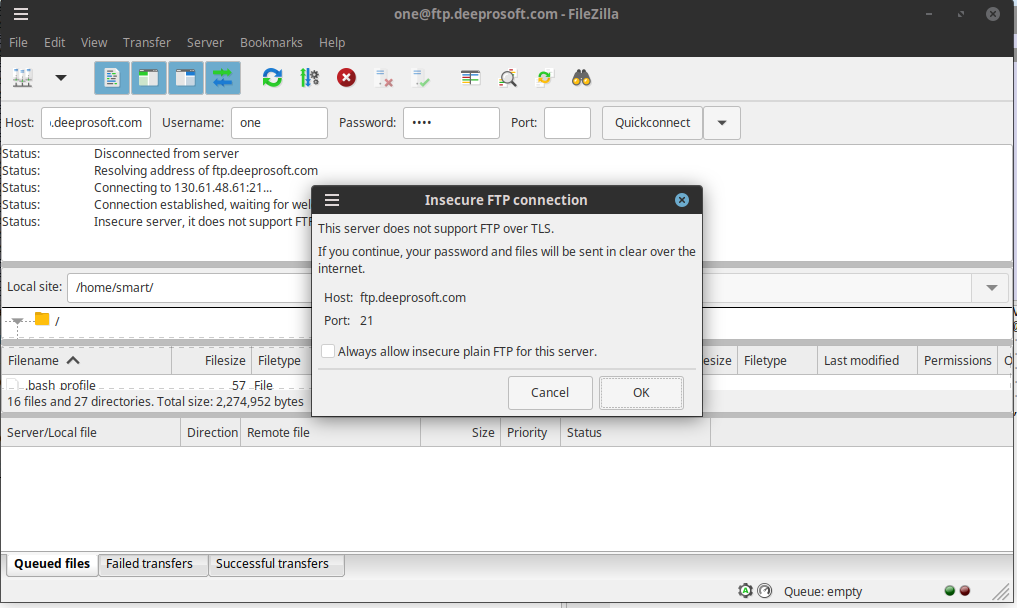
\includegraphics[scale=0.5]{res/5.filezilla-warning.png}
\end{center}

\newpage

При анализе трафика в \texttt{wireshark}, мы видим что со стороны \texttt{filezilla} была попытка установить соединение с использованием \texttt{TLS} и \texttt{SSL}, и только после этого имя пользователя и пароль были переданы в виде чистого текста.
\begin{center}
    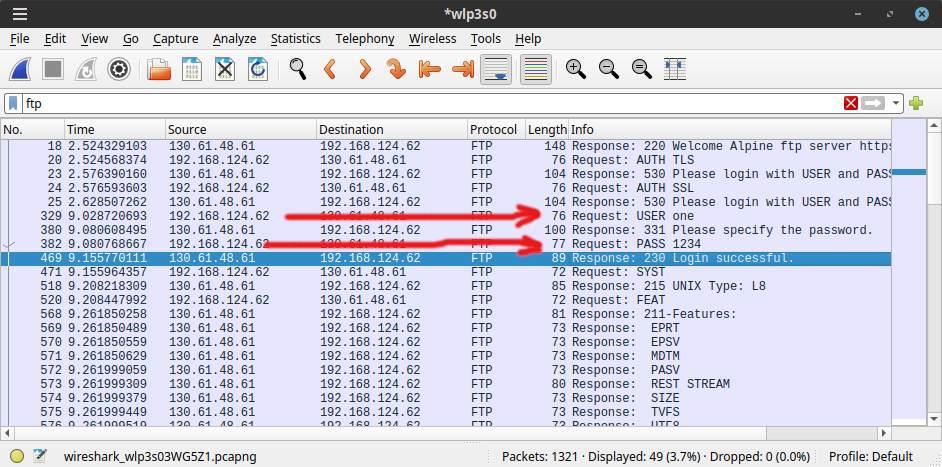
\includegraphics[scale=0.55]{res/5.wireshark-ftp-plain.png}
\end{center}

\subsection*{Шифровние трафика}
\addcontentsline{toc}{subsection}{Шифровние трафика}

Никакие изменения настроек (смена банеров приветствия, отключение анонимного доступа) \texttt{vsftd} не решит проблему передачи логина и пароля в чистом виде. Необходимо организовать обеспечить шифрование канала, а для этого нужно использовать валидные TLS-сертификаты (воспользуемся службой \texttt{LetsEncrypt}).

\begin{Verbatim}[frame=single,breaklines=true,breakanywhere=true]
    ubuntu@temp$ docker run -it --rm \
        -p 80:80 \
        -v "/etc/letsencrypt:/etc/letsencrypt" \
        certbot/certbot certonly \
        --standalone \
        --preferred-challenges http \
        -n --agree-tos \
        --email martynov.sa@edu.spbstu.ru \
        -d ftp.deeprosoft.com
    Unable to find image 'certbot/certbot:latest' locally
    latest: Pulling from certbot/certbot
    ca7dd9ec2225: Pull complete 
    9e124a36b9ab: Pull complete 
    42cba90def7f: Pull complete 
    036c0ab6a768: Pull complete 
    de6312618cf7: Pull complete 
    f2b159e8e18d: Pull complete 
    5c3094a661e9: Pull complete 
    ae4269d8cd1f: Pull complete 
    fc17a613a054: Pull complete 
    7560c853872e: Pull complete 
    ab060fadf2d2: Pull complete 
    b81696353590: Pull complete 
    144b4c29fbe6: Pull complete 
    Digest: sha256:f632e55104da84ba5b54bc858a67ac6c9b4f68790ea823515867c993153c3fb4
    Status: Downloaded newer image for certbot/certbot:latest
    Saving debug log to /var/log/letsencrypt/letsencrypt.log
    Account registered.
    Requesting a certificate for ftp.deeprosoft.com

    Successfully received certificate.
    Certificate is saved at: /etc/letsencrypt/live/ftp.deeprosoft.com/fullchain.pem
    Key is saved at:         /etc/letsencrypt/live/ftp.deeprosoft.com/privkey.pem
    This certificate expires on 2023-05-13.
    These files will be updated when the certificate renews.

    NEXT STEPS:
    - The certificate will need to be renewed before it expires. Certbot can automatically renew the certificate in the background, but you may need to take steps to enable that functionality. See https://certbot.org/renewal-setup for instructions.

    - - - - - - - - - - - - - - - - - - - - - - - - - - - - - - - - - - - - - - - -
    If you like Certbot, please consider supporting our work by:
    * Donating to ISRG / Let's Encrypt:   https://letsencrypt.org/donate
    * Donating to EFF:                    https://eff.org/donate-le
    - - - - - - - - - - - - - - - - - - - - - - - - - - - - - - - - - - - - - - - -
\end{Verbatim}

Теперь запустим \texttt{vsftd}, используя полученные \texttt{TLS}-сертификаты.

\begin{Verbatim}[frame=single,breaklines=true,breakanywhere=true]
    ubuntu@temp$ docker run -d \
        --name ftp \
        -v /etc/letsencrypt:/etc/letsencrypt:ro \
        -p 21:21 \
        -p 21000-21010:21000-21010 \
        -e USERS="one|1234" \
        -e ADDRESS=ftp.deeprosoft.com \
        -e TLS_CERT="/etc/letsencrypt/live/ftp.deeprosoft.com/fullchain.pem" \
        -e TLS_KEY="/etc/letsencrypt/live/ftp.deeprosoft.com/privkey.pem" \
        delfer/alpine-ftp-server
    02c57ccb66c3179da831927af6fe53c29a2ab59926e0901b0fb189ddbc66d06c
\end{Verbatim}

\newpage

Произведём подключение по протоколу \texttt{ftps}.
\begin{center}
    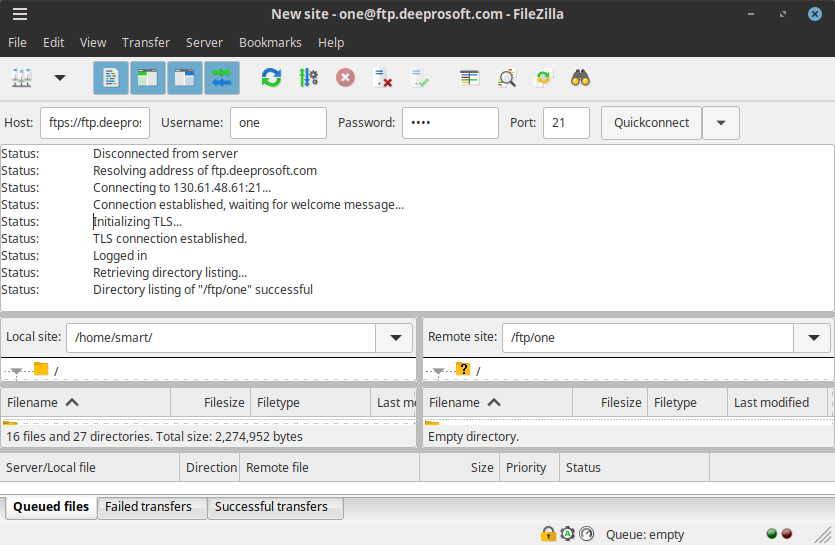
\includegraphics[scale=0.55]{res/5.filezilla-ftps.png}
\end{center}

Снифер \texttt{wireshark} уже не может перехватить пароль.
\begin{center}
    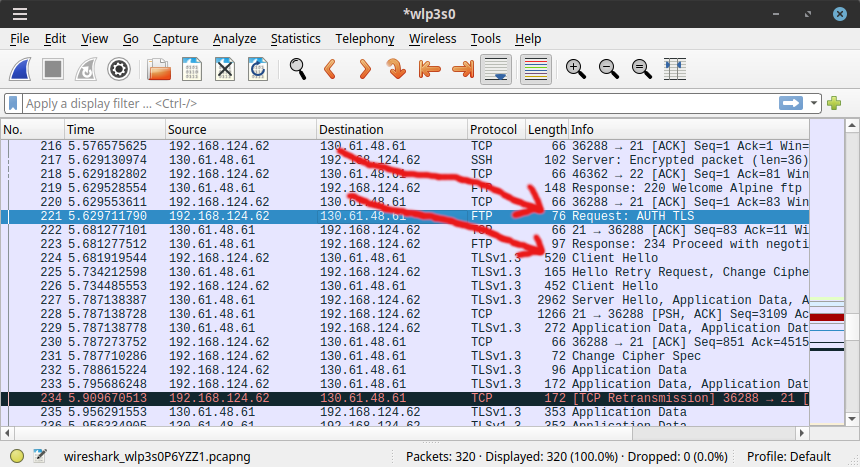
\includegraphics[scale=0.55]{res/5.wireshark-ftps.png}
\end{center}

\newpage

\section*{4. Сравнение защиты Telnet и SSH}
\addcontentsline{toc}{section}{4. Сравнение защиты Telnet и SSH}

Подготовим и запустим \texttt{Telnet} сервер в \texttt{Docker} окружении.
\begin{Verbatim}[frame=single,breaklines=true,breakanywhere=true]
    smart@thinkpad$ docker run -itd -p 23:23 --name=telnetServer flemingcsi/telnet-server
    Unable to find image 'flemingcsi/telnet-server:latest' locally
    latest: Pulling from flemingcsi/telnet-server
    c3b9c0688e3b: Pull complete 
    e9fb5affebb0: Pull complete 
    0f1378f511ad: Pull complete 
    96a961dc7843: Pull complete 
    16564141bc83: Pull complete 
    13bab7266e87: Pull complete 
    Digest: sha256:d667ca1bf508945dffe1de37812bac96469041471f9a1831567cf54004c7e400
    Status: Downloaded newer image for flemingcsi/telnet-server:latest
    066114bb8b7fbb57985e5289bfedc17c5634ac8d9fb2ffaca75bac66b0e075e4
\end{Verbatim}

Уточняю, какой адрес у запущенного сервиса
\begin{Verbatim}[frame=single,breaklines=true,breakanywhere=true]
    smart@thinkpad$ docker inspect --format={{.NetworkSettings.IPAddress}} telnetServer
    172.17.0.2
\end{Verbatim}

Теперь можно воспользоваться \texttt{nc} в качестве \texttt{telnet}-клиента.

При подключении есть какие-то проблемы с кодировкой, но это не важно.

\begin{Verbatim}[frame=single,breaklines=true,breakanywhere=true]
    smart@thinkpad$ nc 127.14.0.2 23
    ???? ?????'username
    password
\end{Verbatim}

\newpage

Снифер \texttt{wireshark} легко перехватывает все сообщения.
\begin{center}
    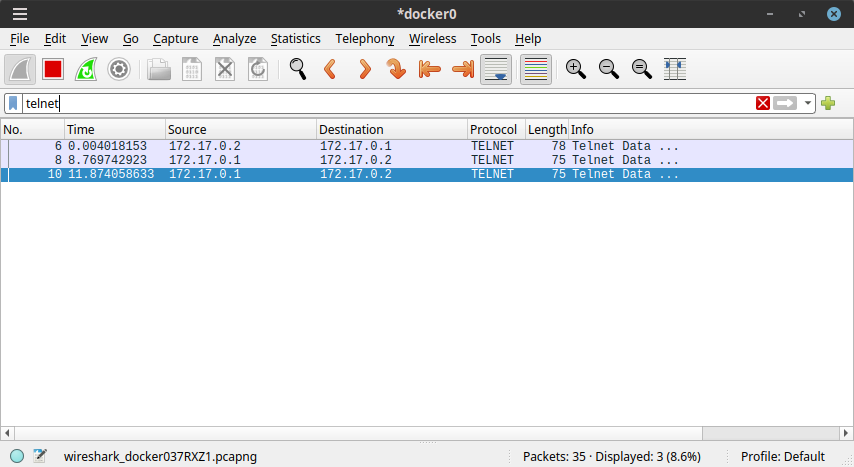
\includegraphics[scale=0.55]{res/5.wireshark-telnet.png}
\end{center}

В меню можно выбрать "Follow TCP stream" для более удобного прочтения перехваченных данных.

Можно без труда получить имя пользователя и пароль, можно просматривать все данные, передаваемые в обе стороны и даже подменять их на лету.

\begin{center}
    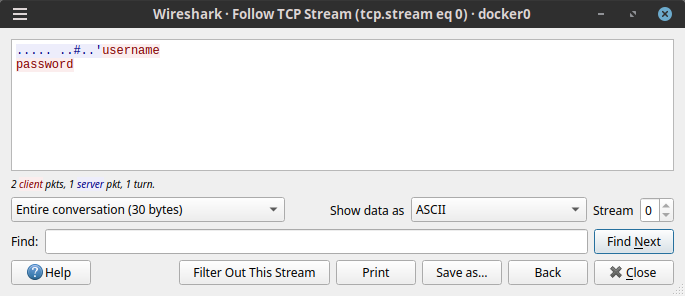
\includegraphics[scale=0.7]{res/5.wireshark-follow-stream.png}
\end{center}

\newpage

При подключении по \texttt{SSH} можно только увидеть \texttt{IP}-адреса клиента и сервера, а так же процесс согласования ключей на эллиптических кривых.

\begin{center}
    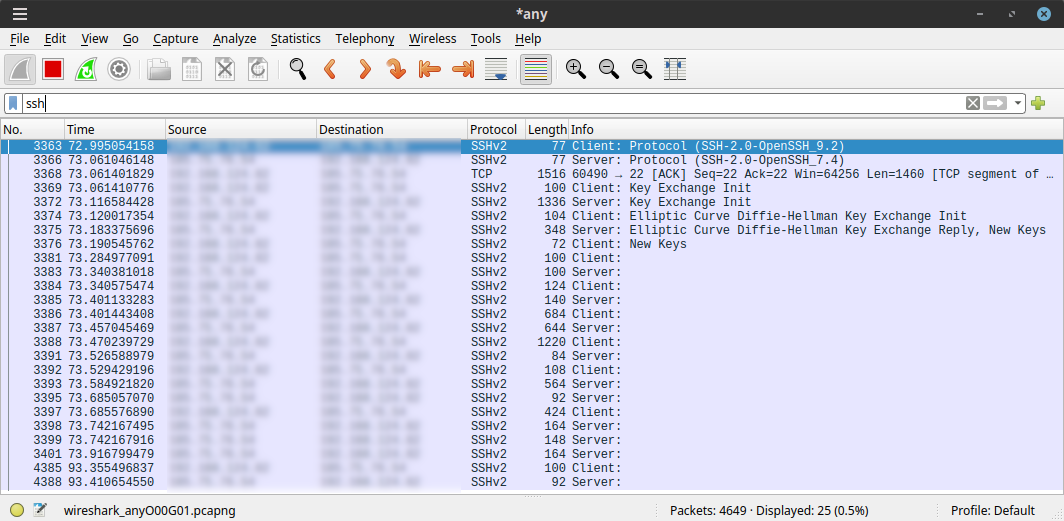
\includegraphics[scale=0.55]{res/5.wireshark-ssh.png}
\end{center}

Просмотреть какой-то трафик не получится, т.к. он надёжно шифруется.

\begin{center}
    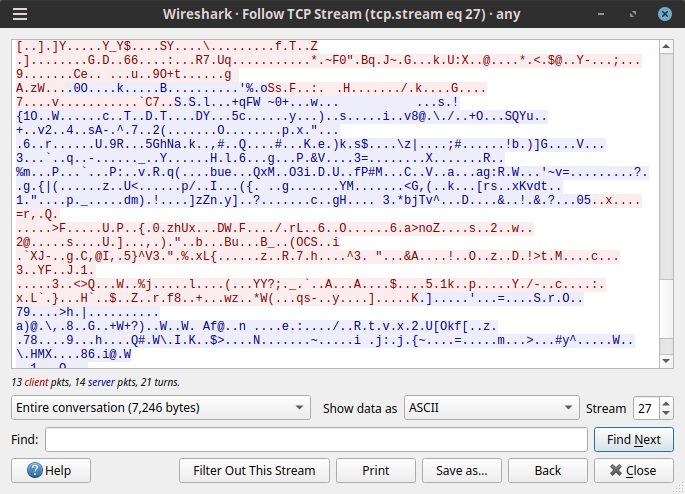
\includegraphics[scale=0.55]{res/5.wireshark-ssh-follow.png}
\end{center}


\section*{5. Анализ сообщений транспортного уровня: UDP-дейтаграммы и TCP-сегменты}
\addcontentsline{toc}{section}{5. Анализ сообщений транспортного уровня: UDP-дейтаграммы и TCP-сегменты}

Все различия происходят из архитектуры этих протоколов.

При фильтрации по \texttt{TCP}, особенно при интенсивном трафике, мы видем большое количество пакетов, связанных с исправлением различных ошибочных ситуаций. При фильтрации по \texttt{UDP} мы видим много пакетов, задача которых в нотификации.

\begin{center}
    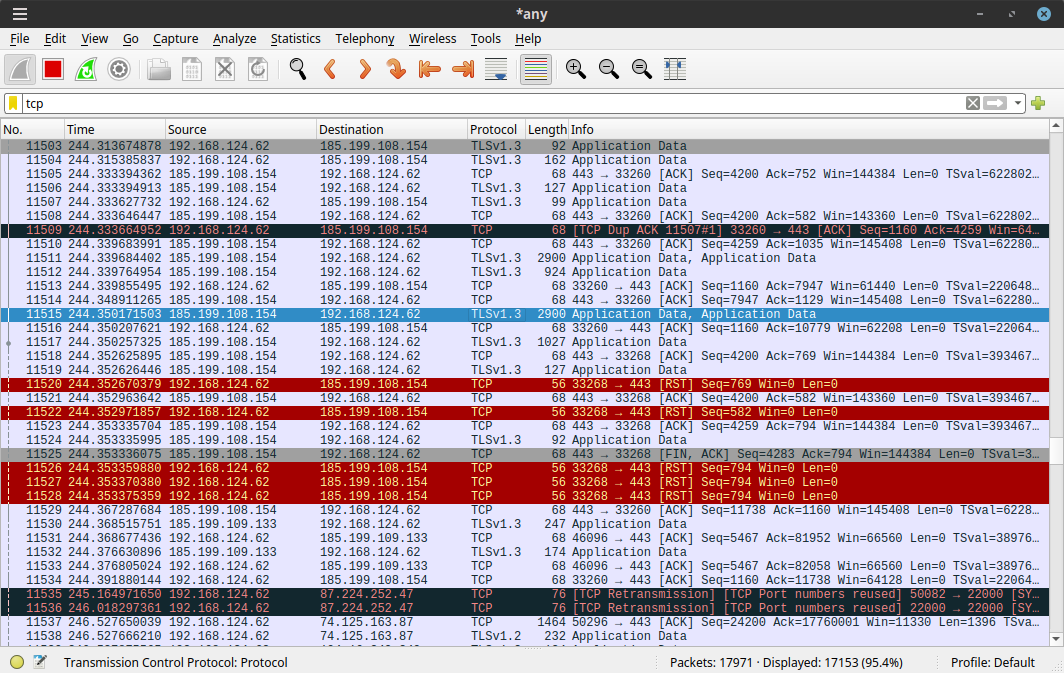
\includegraphics[scale=0.5]{res/5.wireshark-tcp.png}
\end{center}

В каждый пакет данных TCP добавляет заголовок общим объемом в 20 байт (или октетов), в котором содержатся 10 обязательных полей:
\begin{itemize}
    \item Порт источника -- порт устройства-отправителя.
    \item Порт назначения -- порт принимающего устройства.
    \item Порядковый номер -- Устройство, инициирующее TCP-соединение, должно выбрать случайный начальный порядковый номер, который затем увеличивается в соответствии с количеством переданных байтов.
    \item Номер подтверждения -- Принимающее устройство увеличивает этот номер с нуля в соответствии с количеством полученных байтов.
    \item Сдвиг данных TCP -- Данный параметр определяет размер заголовка, чтобы система могла понять, где начинаются данные.
    \item Зарезервированные данные -- зарезервированное поле, значение которого всегда равно нулю. 
    \item Флаги управления -- TCP использует девять флагов для управления потоком данных в определенных ситуациях (например, при инициировании сброса сессии).
    \item Контрольная сумма -- Отправитель генерирует контрольную сумму и передает ее в заголовке каждого пакета. Принимающее устройство может использовать контрольную сумму для проверки ошибок в полученном файле.
    \item Срочный указатель -- это предлагаемая протоколом возможность помечать некоторые байты данных тегом «Срочно» для их пересылки и обработки вне очереди.
    \item Поле опции -- Может использоваться для расширения протокола или его тестирования.
\end{itemize}

\begin{center}
    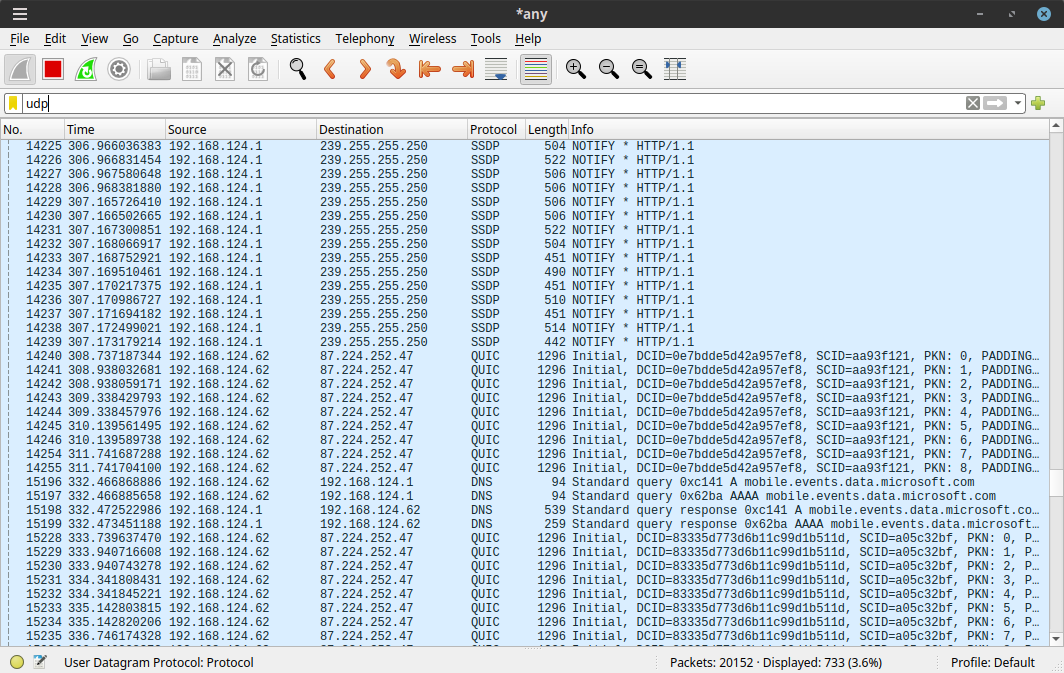
\includegraphics[scale=0.5]{res/5.wireshark-udp.png}
\end{center}

Заголовки UDP значительно проще.
\begin{itemize}
    \item Порт отправителя -- номер порта отправителя
    \item Порт получателя -- содержит порт получателя
    \item Длина датаграммы -- Поле, задающее длину всей датаграммы (заголовка и данных) в байтах. Минимальная длина равна длине заголовка -- 8 байт. Теоретически, максимальный размер поля -- 65535 байт для UDP-датаграммы (8 байт на заголовок и 65527 на данные).
\end{itemize}

\section*{Выводы}
\addcontentsline{toc}{section}{Выводы}

В реальной жизни достаточно тяжело встретиться с такими устаревшими протоколами как \texttt{FTP} или \texttt{Telnet}, но полезно знать об их уязвимостях. В процессе работы использовался сетевой снифер \texttt{wireshark}. На практике инженеры обычно используют \texttt{tcpdump}, но \texttt{wireshark} позволяет легко визуализировать трафик и разложить пакет по битам.

Так же было проведено сравнение между \texttt{TCP} и \texttt{UDP}. Ключевым различием между \texttt{TCP} и \texttt{UDP} является скорость, поскольку \texttt{TCP} сравнительно сложнее \texttt{UDP}. В целом, \texttt{UDP} является быстрым, простым и эффективным протоколом, однако повторная передача потерянных пакетов данных возможна только в \texttt{TCP}.
\chapter*{Лабораторная работа 6. Аудит защищенности сети сканером Nmap}
\addcontentsline{toc}{chapter}{Лабораторная работа 6. Аудит защищенности сети сканером Nmap}

\textbf{Цель работы:} Знакомство с возможностями сетевого сканера Nmap.

\section*{1. Установка}
\addcontentsline{toc}{section}{1. Установка}

Для использования сканера, необходимо произвести установку соответствующего пакета.
\begin{Verbatim}[frame=single]
    smart@thinkpad$ sudo pacman -S nmap
    [sudo] password for smart: 
    resolving dependencies...
    looking for conflicting packages...

    Packages (2) lua53-5.3.6-1  nmap-7.93-1

    Total Download Size:    5.78 MiB
    Total Installed Size:  25.29 MiB

    :: Proceed with installation? [Y/n] 
    :: Retrieving packages...
     lua53-5.3.6-1-x86_64              253.2 KiB   882 KiB/s 00:00 [######################] 100%
     nmap-7.93-1-x86_64                  5.5 MiB  4.33 MiB/s 00:01 [######################] 100%
     Total (2/2)                         5.8 MiB  4.41 MiB/s 00:01 [######################] 100%
    (2/2) checking keys in keyring                                 [######################] 100%
    (2/2) checking package integrity                               [######################] 100%
    (2/2) loading package files                                    [######################] 100%
    (2/2) checking for file conflicts                              [######################] 100%
    (2/2) checking available disk space                            [######################] 100%
    :: Processing package changes...
    (1/2) installing lua53                                         [######################] 100%
    (2/2) installing nmap                                          [######################] 100%
    :: Running post-transaction hooks...
    (1/1) Arming ConditionNeedsUpdate...
\end{Verbatim}

\section*{2. Обнаружение хостов в сети}
\addcontentsline{toc}{section}{2. Обнаружение хостов в сети}

Обрнаружение хостов может стать первым шагом при исследовании сети.

\subsection*{2.1. Наивное сканирование сети}
\addcontentsline{toc}{subsection}{2.1. Наивное сканирование сети}

Выполним сканирование локального сегмента сети с параметрами по умолчанию (иначе, такой вид сканирования называют "наивным").

\begin{Verbatim}[frame=single]
    smart@thinkpad$ nmap 192.168.124.0/24
    Starting Nmap 7.93 ( https://nmap.org ) at 2023-02-13 16:02 MSK
    Nmap scan report for 192.168.124.1
    Host is up (0.0067s latency).
    Not shown: 991 closed tcp ports (conn-refused)
    PORT     STATE SERVICE
    22/tcp   open  ssh
    53/tcp   open  domain
    80/tcp   open  http
    139/tcp  open  netbios-ssn
    222/tcp  open  rsh-spx
    445/tcp  open  microsoft-ds
    1900/tcp open  upnp
    8090/tcp open  opsmessaging
    8200/tcp open  trivnet1

    Nmap scan report for 192.168.124.62
    Host is up (0.00011s latency).
    All 1000 scanned ports on 192.168.124.62 are in ignored states.
    Not shown: 1000 closed tcp ports (conn-refused)

    Nmap scan report for 192.168.124.85
    Host is up (0.033s latency).
    All 1000 scanned ports on 192.168.124.85 are in ignored states.
    Not shown: 1000 closed tcp ports (conn-refused)

    Nmap scan report for 192.168.124.96
    Host is up (0.0044s latency).
    Not shown: 996 closed tcp ports (conn-refused)
    PORT     STATE SERVICE
    1081/tcp open  pvuniwien
    3000/tcp open  ppp
    3001/tcp open  nessus
    9998/tcp open  distinct32

    Nmap scan report for 192.168.124.114
    Host is up (0.018s latency).
    All 1000 scanned ports on 192.168.124.114 are in ignored states.
    Not shown: 1000 closed tcp ports (conn-refused)

    Nmap scan report for 192.168.124.120
    Host is up (0.0050s latency).
    Not shown: 997 closed tcp ports (conn-refused)
    PORT      STATE SERVICE
    49152/tcp open  unknown
    49155/tcp open  unknown
    62078/tcp open  iphone-sync

    Nmap scan report for 192.168.124.131
    Host is up (0.0027s latency).
    Not shown: 998 closed tcp ports (conn-refused)
    PORT      STATE SERVICE
    49152/tcp open  unknown
    62078/tcp open  iphone-sync

    Nmap done: 256 IP addresses (7 hosts up) scanned in 17.14 seconds
\end{Verbatim}

Итого, из 10 устройств, подключенных к роутеру, namp смог опередить 7.

Для каждого обнаруженного хоста, Nmap пытается указывает доменное имя компьютера. Далее Nmap отображает информацию о закрытых или заблокированных портах (Not shown NNNN closed ports), а затем выводит (в три колонки) порты, имеющие другой статус. Первая колонка обозначает текущий номер порта, вторая может принимать различные значения, которые будут свидетельствовать об определенном Nmap статусе порта:

\begin{itemize}
    \item open (открытый порт) -- порт открыт, и служба принимает TCP- или UDP-соединения по этому порту (данный порт наиболее уязвим для взлома);
    \item filtered -- порт закрыт брандмауэром, иной блокирующей программой или службой (правила роутера, аппаратный брандмауэр и т.п.);
    \item closed -- порт закрыт, так как нет службы или иной программы, прослушивающей этот порт на компьютере;
    \item unfiltered, open|filtered или closed|filtered -- Nmap не смог точно определить, открыт порт или закрыт и необходимо использовать сканирование другим методом.
\end{itemize}

Последняя колонка делает предполажение о рабоающем на этом порту сервисе. Допустим, если открыт порт с номером 80, Nmap полагает, что этот порт обычно применяется web-серверами (http). Но это не обязательно так -- практически любой сервис может быть запущен на любом порту, и для более точного определения нужно проводить более глубокое сканирование.

\subsection*{2.2. Обнаружение компьютера методом ping}
\addcontentsline{toc}{subsection}{2.2. Обнаружение компьютера методом ping}

Самым простым является метод обнаружения работающих компьютеров с помощью ping
\begin{Verbatim}[frame=single]
    smart@thinkpad$ nmap -sP 192.168.124.0/24
    Starting Nmap 7.93 ( https://nmap.org ) at 2023-02-13 16:20 MSK
    Nmap scan report for 192.168.124.1
    Host is up (0.0018s latency).
    Nmap scan report for 192.168.124.62
    Host is up (0.000064s latency).
    Nmap scan report for 192.168.124.85
    Host is up (0.044s latency).
    Nmap scan report for 192.168.124.104
    Host is up (0.13s latency).
    Nmap scan report for 192.168.124.114
    Host is up (0.0034s latency).
    Nmap scan report for 192.168.124.130
    Host is up (0.090s latency).
    Nmap scan report for 192.168.124.131
    Host is up (0.084s latency).
    Nmap done: 256 IP addresses (7 hosts up) scanned in 5.73 seconds
\end{Verbatim}

Сетевой сканер Nmap посылает обычные ICMP запросы каждому IP-адресу из списка и ждет ответа. Если ответ получен, значит, сканируемый компьютер работает, что и отображается в качестве результата сканирования. Важно отметить, что удалённый компьютер не обязан отвечать на ICMP запрос, подобные правила легко задаются в фаерволе.

По итогам сканирования мы видим те же 7 хостов. Сканирование было выполнено гораздо быстрее, но не даёт информацию о портах.

\subsection*{2.3. Обнаружение с помощью SYN/ACK- и UDP-пакетов}
\addcontentsline{toc}{subsection}{2.3. Обнаружение с помощью SYN/ACK- и UDP-пакетов}

Для использования флага \texttt{-PU} (UDP ping) требуется root-доступ, т.к. требуется доступ к сырому ответу с канального уровня.

\begin{Verbatim}[frame=single]
    smart@thinkpad$ sudo nmap -PS80 -PU -PA -PY 192.168.124.0/24
    [sudo] password for smart: 
    Starting Nmap 7.93 ( https://nmap.org ) at 2023-02-13 16:27 MSK
    Nmap scan report for 192.168.124.1
    Host is up (0.0020s latency).
    Not shown: 991 closed tcp ports (reset)
    PORT     STATE SERVICE
    22/tcp   open  ssh
    53/tcp   open  domain
    80/tcp   open  http
    139/tcp  open  netbios-ssn
    222/tcp  open  rsh-spx
    445/tcp  open  microsoft-ds
    1900/tcp open  upnp
    8090/tcp open  opsmessaging
    8200/tcp open  trivnet1
    MAC Address: 34:CE:00:37:D9:03 (Xiaomi Electronics,co.)

    Nmap scan report for 192.168.124.85
    Host is up (0.028s latency).
    All 1000 scanned ports on 192.168.124.85 are in ignored states.
    Not shown: 1000 closed tcp ports (reset)
    MAC Address: 34:CE:00:86:A0:C4 (Xiaomi Electronics,co.)

    Nmap scan report for 192.168.124.104
    Host is up (0.0047s latency).
    All 1000 scanned ports on 192.168.124.104 are in ignored states.
    Not shown: 1000 closed tcp ports (reset)
    MAC Address: 34:CE:00:BD:11:0F (Xiaomi Electronics,co.)

    Nmap scan report for 192.168.124.114
    Host is up (0.0061s latency).
    All 1000 scanned ports on 192.168.124.114 are in ignored states.
    Not shown: 1000 closed tcp ports (reset)
    MAC Address: 34:CE:00:86:67:69 (Xiaomi Electronics,co.)

    Nmap scan report for 192.168.124.131
    Host is up (0.0027s latency).
    Not shown: 998 closed tcp ports (reset)
    PORT      STATE SERVICE
    49152/tcp open  unknown
    62078/tcp open  iphone-sync
    MAC Address: 2E:0E:A4:CF:16:E1 (Unknown)

    Nmap scan report for 192.168.124.132
    Host is up (0.0064s latency).
    Not shown: 997 closed tcp ports (reset)
    PORT      STATE SERVICE
    49152/tcp open  unknown
    49153/tcp open  unknown
    62078/tcp open  iphone-sync
    MAC Address: D6:F0:D3:73:71:73 (Unknown)

    Nmap scan report for 192.168.124.62
    Host is up (0.0000040s latency).
    All 1000 scanned ports on 192.168.124.62 are in ignored states.
    Not shown: 1000 closed tcp ports (reset)

    Nmap done: 256 IP addresses (7 hosts up) scanned in 14.89 seconds
\end{Verbatim}

Если какой-либо сервис прослушивает порт, а Nmap пытается установить соединение с ним (отсылает пакет с флагом \texttt{SYN}), в ответ сервис может послать пакет с флагами \texttt{SYN/ACK}, что покажет: компьютер в сети существует.

При отсутствии сервиса по этому порту сервер посылает в ответ пакет с флагом \texttt{RST}, что также указывает, что по заданному IP-адресу компьютер есть.

Если в ответ на посланный пакет SYN от сервера ничего не пришло — это значит, что либо компьютер выключен, либо трафик блокируется брандмауэром. Чтобы обойти блокирование брандмауэром, разработан еще один метод сканирования. Сканер Nmap обычно посылает пакеты с флагами \texttt{SYN/ACK} и пакет UDP по стандартному 80-му порту, который чаще всего используется для web-трафика и поэтому очень редко блокируется брандмауэром.

\begin{itemize}
    \item \texttt{-PS} -- TCP SYN
    \item \texttt{-PA} -- TCP ACK
    \item \texttt{-PU} -- UDP
    \item \texttt{-PY} -- SCTP
\end{itemize}

\subsection*{2.4. Обнаружение компьютера посредством различных ICMP-пакетов}
\addcontentsline{toc}{subsection}{2.4. Обнаружение компьютера посредством различных ICMP-пакетов}

Ранее мы использовали простой ICMP-запрос, но такой трафик может быть заблокирован. У сетевого сканера Nmap есть другие возможности определения хоста при помощи ICMP.


\begin{Verbatim}[frame=single]
    smart@thinkpad$ sudo nmap -PE -PP -PM 192.168.124.0/24
    Starting Nmap 7.93 ( https://nmap.org ) at 2023-02-13 16:49 MSK
    Nmap scan report for 192.168.124.1
    Host is up (0.0047s latency).
    Not shown: 991 closed tcp ports (reset)
    PORT     STATE SERVICE
    22/tcp   open  ssh
    53/tcp   open  domain
    80/tcp   open  http
    139/tcp  open  netbios-ssn
    222/tcp  open  rsh-spx
    445/tcp  open  microsoft-ds
    1900/tcp open  upnp
    8090/tcp open  opsmessaging
    8200/tcp open  trivnet1
    MAC Address: 34:CE:00:37:D9:03 (Xiaomi Electronics,co.)

    Nmap scan report for 192.168.124.62
    Host is up (0.000012s latency).
    All 1000 scanned ports on 192.168.124.62 are in ignored states.
    Not shown: 1000 closed tcp ports (reset)

    Nmap done: 256 IP addresses (2 hosts up) scanned in 3.38 seconds
\end{Verbatim}

Рассмотрим дополнительные ключи:
\begin{itemize}
    \item \texttt{-PE} -- ICMP echo, уже использовали ранее
    \item \texttt{-PP} -- ICMP timestamp requests, запрос времени
    \item \texttt{-PM} -- ICMP netmask request discovery, запрос адреса и маски
\end{itemize}
С помощью этих методов тоже можно получить ответ от удаленного компьютера.

\section*{3. Сканирование портов}
\addcontentsline{toc}{section}{3. Сканирование портов}

Многие методы задействуют различные манипуляции с флагами TCP-пакетов на низком уровне, а потому для работы требуют полномочий root (суперпользователя) в системе.

\subsection*{3.1. Сканирование портов методом SYN}
\addcontentsline{toc}{subsection}{3.1. Сканирование портов методом SYN}

Наиболее распространенный метод, который используется по умолчанию, — это сканирование TCP SYN. Этот подход позволяет сканировать несколько сотен портов в секунду, скрывая при этом сканирующий компьютер, поскольку никогда не завершает TCP-соединение.

\begin{Verbatim}[frame=single]
    smart@thinkpad$ sudo nmap -sS 192.168.124.0/24
    Starting Nmap 7.93 ( https://nmap.org ) at 2023-02-13 17:03 MSK
    Nmap scan report for 192.168.124.1
    Host is up (0.0013s latency).
    Not shown: 991 closed tcp ports (reset)
    PORT     STATE SERVICE
    22/tcp   open  ssh
    53/tcp   open  domain
    80/tcp   open  http
    139/tcp  open  netbios-ssn
    222/tcp  open  rsh-spx
    445/tcp  open  microsoft-ds
    1900/tcp open  upnp
    8090/tcp open  opsmessaging
    8200/tcp open  trivnet1
    MAC Address: 34:CE:00:37:D9:03 (Xiaomi Electronics,co.)

    Nmap scan report for 192.168.124.53
    Host is up (0.039s latency).
    All 1000 scanned ports on 192.168.124.53 are in ignored states.
    Not shown: 1000 filtered tcp ports (no-response)
    MAC Address: 1C:91:80:CE:C8:F4 (Apple)

    Nmap scan report for 192.168.124.96
    Host is up (0.0017s latency).
    Not shown: 996 closed tcp ports (reset)
    PORT     STATE SERVICE
    1081/tcp open  pvuniwien
    3000/tcp open  ppp
    3001/tcp open  nessus
    9998/tcp open  distinct32
    MAC Address: 38:8C:50:52:42:D7 (LG Electronics)

    Nmap scan report for 192.168.124.104
    Host is up (0.034s latency).
    All 1000 scanned ports on 192.168.124.104 are in ignored states.
    Not shown: 1000 closed tcp ports (reset)
    MAC Address: 34:CE:00:BD:11:0F (Xiaomi Electronics,co.)

    Nmap scan report for 192.168.124.114
    Host is up (0.044s latency).
    All 1000 scanned ports on 192.168.124.114 are in ignored states.
    Not shown: 1000 closed tcp ports (reset)
    MAC Address: 34:CE:00:86:67:69 (Xiaomi Electronics,co.)

    Nmap scan report for 192.168.124.120
    Host is up (0.0055s latency).
    Not shown: 997 closed tcp ports (reset)
    PORT      STATE SERVICE
    49152/tcp open  unknown
    49155/tcp open  unknown
    62078/tcp open  iphone-sync
    MAC Address: 6E:63:9D:97:70:7F (Unknown)

    Nmap scan report for 192.168.124.62
    Host is up (0.0000050s latency).
    All 1000 scanned ports on 192.168.124.62 are in ignored states.
    Not shown: 1000 closed tcp ports (reset)

    Nmap done: 256 IP addresses (7 hosts up) scanned in 40.58 seconds
\end{Verbatim}

Сканер Nmap отправляет исследуемому компьютеру пакет с флагом \texttt{SYN}, как будто он хочет открыть обычное TCP-соединение, следуя приведенным в начале статьи правилам. Если ответ (пакет с флагами \texttt{SYN/ACK}) от запрашиваемого хоста получен, порт будет обозначен как открытый, а при получении пакета с флагом \texttt{RST} -- как закрытый. В случае если сканируемый компьютер не ответил, предполагается, что этот порт фильтруется брандмауэром.

\subsection*{3.2. Сканирование с использованием системной функции connect()}
\addcontentsline{toc}{subsection}{3.2. Сканирование с использованием системной функции connect()}

Метод, основанный на установлении соединения с помощью системной функции \texttt{connect()}, которую применяет большинство приложений.

\begin{Verbatim}[frame=single]
    smart@thinkpad$ nmap -sT 192.168.124.0/24
    Starting Nmap 7.93 ( https://nmap.org ) at 2023-02-13 17:03 MSK
    Nmap scan report for 192.168.124.1
    Host is up (0.0076s latency).
    Not shown: 991 closed tcp ports (conn-refused)
    PORT     STATE SERVICE
    22/tcp   open  ssh
    53/tcp   open  domain
    80/tcp   open  http
    139/tcp  open  netbios-ssn
    222/tcp  open  rsh-spx
    445/tcp  open  microsoft-ds
    1900/tcp open  upnp
    8090/tcp open  opsmessaging
    8200/tcp open  trivnet1

    Nmap scan report for 192.168.124.62
    Host is up (0.00014s latency).
    All 1000 scanned ports on 192.168.124.62 are in ignored states.
    Not shown: 1000 closed tcp ports (conn-refused)

    Nmap scan report for 192.168.124.85
    Host is up (0.034s latency).
    All 1000 scanned ports on 192.168.124.85 are in ignored states.
    Not shown: 1000 closed tcp ports (conn-refused)

    Nmap scan report for 192.168.124.96
    Host is up (0.0040s latency).
    Not shown: 996 closed tcp ports (conn-refused)
    PORT     STATE SERVICE
    1081/tcp open  pvuniwien
    3000/tcp open  ppp
    3001/tcp open  nessus
    9998/tcp open  distinct32

    Nmap scan report for 192.168.124.104
    Host is up (0.0062s latency).
    All 1000 scanned ports on 192.168.124.104 are in ignored states.
    Not shown: 1000 closed tcp ports (conn-refused)

    Nmap scan report for 192.168.124.114
    Host is up (0.0067s latency).
    All 1000 scanned ports on 192.168.124.114 are in ignored states.
    Not shown: 1000 closed tcp ports (conn-refused)

    Nmap done: 256 IP addresses (6 hosts up) scanned in 26.51 seconds
\end{Verbatim}

Запрос отправляется операционной системе, которая устанавливает TCP-соединение. После определения статуса порта Nmap прерывает соединение, то есть с помощью функции \texttt{connect()} посылается пакет с флагом \texttt{RST}.

Отрицательной стороной является то, что подобный способ логируется в системных журналах, раскрывая факт сканирования.

\subsection*{3.3. Сканирование портов UDP-протокола}
\addcontentsline{toc}{subsection}{3.3. Сканирование портов UDP-протокола}

Наиболее распространенные сервисы, использующие UDP-протокол это DNS, SNMP и DHCP.

\begin{Verbatim}[frame=single]
    smart@thinkpad$ sudo nmap -sU -sV 192.168.124.1
    [sudo] password for smart: 
    Starting Nmap 7.93 ( https://nmap.org ) at 2023-02-13 17:28 MSK
    Nmap scan report for 192.168.124.1
    Host is up (0.0020s latency).
    Not shown: 991 closed udp ports (port-unreach)
    PORT     STATE         SERVICE      VERSION
    53/udp   open          domain       ISC BIND 9.8.4-rpz2+rl005.12-P1
    67/udp   open|filtered dhcps
    137/udp  open          netbios-ns   Microsoft Windows netbios-ns (workgroup: WORKGROUP)
    138/udp  open|filtered netbios-dgm
    1900/udp open          upnp?
    3702/udp open|filtered ws-discovery
    5351/udp open          nat-pmp?
    5353/udp open          mdns         DNS-based service discovery
    5355/udp open|filtered llmnr
    1 service unrecognized despite returning data. If you know the service/version, please submit the following fingerprint at https://nmap.org/cgi-bin/submit.cgi?new-service :
    SF-Port5351-UDP:V=7.93%I=7%D=2/13%Time=63EA4D46%P=x86_64-pc-linux-gnu%r(DN
    SF:SVersionBindReq,8,"\0\x86\0\x05\x003\x7fy")%r(DNSStatusRequest,C,"\0\x8
    SF:0\0\0\x003\x7f~\xbc\xe3\*\$")%r(Help,18,"\0\xe5\0\x03\0\0\0\0\x003\x7f\
    SF:x88\0\0\0\0\0\0\0\0\0\0\0\0")%r(SIPOptions,E8,"\0\xd0\0\x03\0\0\0\0\x00
    SF:3\x7f\x8d\0\0\0\0\0\0\0\0\0\0\0\0Via:\x20SIP/2\.0/UDP\x20nm;branch=foo;
    SF:rport\r\nFrom:\x20<sip:nm@nm>;tag=root\r\nTo:\x20<sip:nm2@nm2>\r\nCall-
    SF:ID:\x2050000\r\nCSeq:\x2042\x20OPTIONS\r\nMax-Forwards:\x2070\r\nConten
    SF:t-Length:\x200\r\nContact:\x20<sip:nm@nm>\r\nAccept:\x20application/sdp
    SF:\r\n\r\n\0\0\0")%r(NTPRequest,30,"\x02\x80\0\x01\0\0\0\0\x003\x7f\x9a\0
    SF:\0\0\0\0\0\0\0\0\0\0\0\0\0\0\0\0\0\0\0\0\0\0\0\0\0\0\0\xc5O#Kq\xb1R\xf3
    SF:")%r(SNMPv3GetRequest,3C,"\x02\xba\0\x01\0\0\0\0\x003\x7f\xa4\0\0\0\0\0
    SF:\0\0\0\0\0\0\x000\x0e\x04\0\x02\x01\0\x02\x01\0\x04\0\x04\0\x04\x000\x1
    SF:2\x04\0\x04\0\xa0\x0c\x02\x027\xf0\x02\x01\0\x02\x01\x000\0")%r(AFSVers
    SF:ionRequest,C,"\0\x80\0\0\x003\x7f\xae\xbc\xe3\*\$")%r(DNS-SD,C,"\0\x80\
    SF:0\0\x003\x7f\xb3\xbc\xe3\*\$")%r(Citrix,20,"\0\x80\0\x03\0\0\0\0\x003\x
    SF:7f\xb8\0\0\0\0\0\0\0\0\0\0\0\0\0\0\0\0\0\0\0\0")%r(sybaseanywhere,40,"\
    SF:0\x80\0\x03\0\0\0\0\x003\x7f\xc2\0\0\0\0\0\0\0\0\0\0\0\0TDS\0\0\0\x01\0
    SF:\0\x04\0\x05\0\x05\0\0\x01\x02\0\0\x03\x01\x01\x04\x08\0\0\0\0\0\0\0\0\
    SF:x07\x02\x04\xb1\0\0\0")%r(NetMotionMobility,8,"\0\xc0\0\x05\x003\x7f\xc
    SF:7");
    MAC Address: 34:CE:00:37:D9:03 (Xiaomi Electronics,co.)
    Service Info: Host: KEENETIC; OS: Windows; CPE: cpe:/o:microsoft:windows

    Service detection performed. Please report any incorrect results at https://nmap.org/submit/ .
    Nmap done: 1 IP address (1 host up) scanned in 1141.84 seconds
\end{Verbatim}

Процесс сканирования занял много времени, и в итоге был обнаружен сервис, про который Namp ничего не знает, и предлагает отправить отчёт разработчикам.

Метод сканирования UDP отличается от рассмотренных методов TCP. Nmap посылает UDP-пакет с пустым заголовком по всем исследуемым портам и ждет ответа. Если в ответ он получает ICMP-пакет с ошибкой \texttt{unreachable error}, порт считается закрытым. При получении пакетов с другими ошибками Nmap считает, что порт фильтруется брандмауэром. Полученный ответный UDP-пакет свидетельствует о наличии сервиса, и порт маркируется открытым. Если ответ не получен после нескольких попыток, Nmap помечает порт как \texttt{open|filtered}, поскольку не может точно установить — открыт ли порт или брандмауэр блокирует трафик на этом порту.

Рассмотрим ключи:
\begin{itemize}
    \item \texttt{-sU} -- Сам запуск UPD сканирования
    \item \texttt{-sV} -- Определить версию запущенного сервиса (существенно увеличивает время сканирования)
\end{itemize}

\subsection*{3.4. Сканирование с помощью методов FIN, Xmas и Null}
\addcontentsline{toc}{subsection}{3.4. Сканирование с помощью методов FIN, Xmas и Null}

Прерывания последовательности соединения можно также получить информацию о закрытых и открытых портах исследуемого хоста.

\begin{Verbatim}[frame=single]
    smart@thinkpad$ sudo nmap -sF 192.168.124.1
    Starting Nmap 7.93 ( https://nmap.org ) at 2023-02-13 17:26 MSK
    Nmap scan report for 192.168.124.1
    Host is up (0.0013s latency).
    All 1000 scanned ports on 192.168.124.1 are in ignored states.
    Not shown: 1000 open|filtered tcp ports (no-response)
    MAC Address: 34:CE:00:37:D9:03 (Xiaomi Electronics,co.)

    Nmap done: 1 IP address (1 host up) scanned in 21.34 seconds

    smart@thinkpad$ sudo nmap -sN 192.168.124.1
    Starting Nmap 7.93 ( https://nmap.org ) at 2023-02-13 17:26 MSK
    Nmap scan report for 192.168.124.1
    Host is up (0.0017s latency).
    All 1000 scanned ports on 192.168.124.1 are in ignored states.
    Not shown: 1000 open|filtered tcp ports (no-response)
    MAC Address: 34:CE:00:37:D9:03 (Xiaomi Electronics,co.)

    Nmap done: 1 IP address (1 host up) scanned in 21.29 seconds

    smart@thinkpad$ sudo nmap -sX 192.168.124.1
    Starting Nmap 7.93 ( https://nmap.org ) at 2023-02-13 17:27 MSK
    Nmap scan report for 192.168.124.1
    Host is up (0.0017s latency).
    All 1000 scanned ports on 192.168.124.1 are in ignored states.
    Not shown: 1000 open|filtered tcp ports (no-response)
    MAC Address: 34:CE:00:37:D9:03 (Xiaomi Electronics,co.)

    Nmap done: 1 IP address (1 host up) scanned in 21.27 seconds
\end{Verbatim}

Рассмотрим эти методы сканирования
\begin{itemize}
    \item \texttt{-sF} FIN-сканирование -- удаленному хосту посылаются пакеты с флагом \texttt{FIN}, которые обычно применяются при закрытии соединения. В этом случае закрытый порт компьютера, в соответствии со спецификацией протокола TCP, должен послать ответный пакет с флагом \texttt{RST}. Если же порт открыт или блокируется брандмауэром, ответа от него не будет.
    \item \texttt{-sN} null-сканирование -- та же самая механика, но вместо пакета с \texttt{FIN}-флагом отсылается пакет с пустым заголовком (0 бит, все флаги отключены).
    \item \texttt{-sX} Xmas-сканирование -- та же механика, но хосту отсылается пакет, раскрашенный несколькими флагами (\texttt{FIN}, \texttt{PSH} и \texttt{URG}) на манер рождественской елки.
\end{itemize}

\subsection*{3.5. Сканирование с помощью методов ACK и Window}
\addcontentsline{toc}{subsection}{3.5. Сканирование с помощью методов ACK и Window}

Для определения, какие порты на компьютере находятся в статусе \texttt{filtered}, а какие в \texttt{unfiltered}, существует отдельно вынесенный тип сканирования.

\begin{Verbatim}[frame=single]
    smart@thinkpad$ sudo nmap -sA 192.168.124.1
    Starting Nmap 7.93 ( https://nmap.org ) at 2023-02-13 18:28 MSK
    Nmap scan report for 192.168.124.1
    Host is up (0.0055s latency).
    All 1000 scanned ports on 192.168.124.1 are in ignored states.
    Not shown: 1000 unfiltered tcp ports (reset)
    MAC Address: 34:CE:00:37:D9:03 (Xiaomi Electronics,co.)
    
    Nmap done: 1 IP address (1 host up) scanned in 0.37 seconds
\end{Verbatim}

Многие фаерволы выполняют проверку только \texttt{SYN}-пакетов на определенном порту, осуществляя тем самым фильтрацию, с помощью отсылки пакетов с флагом \texttt{ACK} можно определить, существует ли на удалённом компьютере брандмауэр или нет. Пакет с флагом \texttt{ACK} в этом случае отсылается не как часть соединения, а отдельно. В случае если принимающая сторона отсылает обратный пакет с флагом \texttt{RST} (соответственно порт не блокируется брандмауэром), порт помечается как \texttt{unfiltered}, если же хост не отвечает на пакет, то на нем установлен брандмауэр и порт находится в статусе \texttt{filtered}.

\begin{Verbatim}[frame=single]
    smart@thinkpad$ sudo nmap -sW 192.168.124.1
    Starting Nmap 7.93 ( https://nmap.org ) at 2023-02-13 18:29 MSK
    Nmap scan report for 192.168.124.1
    Host is up (0.0076s latency).
    All 1000 scanned ports on 192.168.124.1 are in ignored states.
    Not shown: 1000 closed tcp ports (reset)
    MAC Address: 34:CE:00:37:D9:03 (Xiaomi Electronics,co.)

    Nmap done: 1 IP address (1 host up) scanned in 0.39 seconds
\end{Verbatim}

Существует аналогичный метод, который работает по такому же принципу, но иначе интерпретирует полученные от хоста результаты. Сканирование методом \texttt{TCP Window} предполагает, что на некоторых хостах службы используют положительное значение поля \texttt{window} в ответном пакете (не ноль). Поэтому с помощью данного метода Nmap анализирует заголовки приходящих пакетов с флагом \texttt{RST}, и если приходящий пакет содержит положительное значение поля, то Nmap помечает этот порт открытым. Получение пакета с нулевым значением поля означает, что порт закрыт.

В нашем случае фаервол на удалённом хосте не обнаружен.

\subsection*{3.6. Сканирование методом Maimon}
\addcontentsline{toc}{subsection}{3.6. Сканирование методом Maimon}

Способ сканирования был предложен специалистом, по имени Uriel Maimon.

Механика метода сходна с \texttt{FIN}, \texttt{Xmas} и \texttt{Null}, но отправляются пакеты с флагами \texttt{FIN/ACK}. Если порт закрыт, хост должен отвечать пакетом \texttt{RST}.

\begin{Verbatim}[frame=single]
    smart@thinkpad$ sudo nmap -sM 192.168.124.1
    Starting Nmap 7.93 ( https://nmap.org ) at 2023-02-13 18:48 MSK
    Nmap scan report for 192.168.124.1
    Host is up (0.0016s latency).
    Not shown: 998 open|filtered tcp ports (no-response)
    PORT    STATE  SERVICE
    139/tcp closed netbios-ssn
    445/tcp closed microsoft-ds
    MAC Address: 34:CE:00:37:D9:03 (Xiaomi Electronics,co.)

    Nmap done: 1 IP address (1 host up) scanned in 4.65 seconds
\end{Verbatim}

\subsection*{3.7. Скрытое сканирование с использованием алгоритма idlescan}
\addcontentsline{toc}{subsection}{3.7. Скрытое сканирование с использованием алгоритма idlescan}

Метод idlescan по своему алгоритму работы практически идентичен SYN-сканированию, но пытается скрыть IP-адрес хоста, с которого производится исследование.

Попытка просканировать хост 192.168.124.1 выдавая себя за хост 192.168.124.96.
\begin{Verbatim}[frame=single]
    smart@thinkpad$ sudo nmap -sI 192.168.124.96 192.168.124.1
    WARNING: Many people use -Pn w/Idlescan to prevent pings from their true IP.  On the other hand, timing info Nmap gains from pings can allow for faster, more reliable scans.
    Starting Nmap 7.93 ( https://nmap.org ) at 2023-02-13 18:56 MSK
    Idle scan using zombie 192.168.124.96 (192.168.124.96:443); Class: Incremental
    Idle scan is unable to obtain meaningful results from proxy 192.168.124.96 (192.168.124.96).  I'm sorry it didn't work out.
    QUITTING!
\end{Verbatim}

Результаты такого сканирования часто бывают не точны, при этом требуют довольно много времени. В нашем случае никакие полезные результаты получить не удалось.

\subsection*{3.8. Сканирование на наличие открытых протоколов}
\addcontentsline{toc}{subsection}{3.8. Сканирование на наличие открытых протоколов}

Иногда достаточно просто определить сам факт наличия открытого порта на удалённом хосте.

Для определения доступности протокола на хосте Nmap посылает несколько пакетов с пустыми заголовками, содержащими в поле protocol только номер протокола. В случае, если протокол недоступен, компьютер вернет ICMP-сообщение «protocol unreachable». Если в ответ хост не посылает пакетов -- это может означать, что либо протокол доступен, либо брандмауэр блокирует ICMP-трафик.

\begin{Verbatim}[frame=single]
    smart@thinkpad$ sudo nmap -sO 192.168.124.1
    Starting Nmap 7.93 ( https://nmap.org ) at 2023-02-13 18:58 MSK
    Nmap scan report for 192.168.124.1
    Host is up (0.0029s latency).
    Not shown: 245 closed n/a protocols (proto-unreach)
    PROTOCOL STATE         SERVICE
    1        open          icmp
    2        open|filtered igmp
    4        open|filtered ipv4
    6        open          tcp
    17       open          udp
    41       open|filtered ipv6
    47       open|filtered gre
    50       open|filtered esp
    51       open|filtered ah
    108      open|filtered ipcomp
    136      open|filtered udplite
    MAC Address: 34:CE:00:37:D9:03 (Xiaomi Electronics,co.)

    Nmap done: 1 IP address (1 host up) scanned in 322.60 seconds
\end{Verbatim}

\subsection*{3.9. Скрытное сканирование посредством метода ftp bounce}
\addcontentsline{toc}{subsection}{3.9. Скрытное сканирование посредством метода ftp bounce}

Метод основан на возможности FTP-сервера отправлять файлы 3й стороне. Зная об этой уязвимости, многие владельцы FTP-серверов закрыли эту возможность.

В нашей сети нет FTP-сервера, но мы просто упоминаем эту возможность как опцию для сканирования.

\begin{Verbatim}[frame=single]
    smart@thinkpad$ sudo nmap -b <username:password@server:port> 192.168.124.1
\end{Verbatim}

\section*{4. Изучение служб на удалёных хостах}
\addcontentsline{toc}{section}{4. Изучение служб на удалёных хостах}

Nmap с большой степенью вероятности позволяет определять версию операционной системы, которая запущена на удаленном компьютере. При этом Nmap может также идентифицировать версии запущенных на удаленном ПК сервисов, при условии что порты того или иного сервиса открыты.

\subsection*{4.1. Определение версии ОС}
\addcontentsline{toc}{subsection}{4.1. Определение версии ОС}

Сканер Nmap собирает "отпечатки пальцев" (fingerprints) различных хостов и запущенных там сервисов. Сравнивая полученные результаты с эталонными значениями, указанными в файле Nmap-os-fingerprints, программа выдает сводный результат по компьютеру.

\begin{Verbatim}[frame=single]
    smart@thinkpad$ sudo nmap -O -A 192.168.124.96
    Starting Nmap 7.93 ( https://nmap.org ) at 2023-02-13 19:24 MSK
    Nmap scan report for 192.168.124.96
    Host is up (0.0020s latency).
    Not shown: 996 closed tcp ports (reset)
    Bug in uptime-agent-info: no string output.
    PORT     STATE SERVICE  VERSION
    1081/tcp open  upnp     Platinum unpnd 1.0.4.9 (arch: i686; UPnP 1.0; DLNADOC 1.50)
    3000/tcp open  http     LG smart TV http service
    |_http-title: Site doesn't have a title.
    3001/tcp open  ssl/http LG smart TV http service
    | tls-nextprotoneg: 
    |   http/1.1
    |_  http/1.0
    |_http-title: Site doesn't have a title.
    |_ssl-date: TLS randomness does not represent time
    | ssl-cert: Subject: commonName=LG_TV_1ba52211ee27c01/organizationName=LG Electronics U.S.A, Inc./stateOrProvinceName=New Jersey/countryName=US
    | Not valid before: 2018-11-11T07:30:39
    |_Not valid after:  2038-11-06T07:30:39
    9998/tcp open  http     Google Chromecast httpd
    |_http-title: Cast shell remote debugging
    MAC Address: 38:8C:50:52:42:D7 (LG Electronics)
    Device type: general purpose
    Running: Linux 3.X|4.X
    OS CPE: cpe:/o:linux:linux_kernel:3 cpe:/o:linux:linux_kernel:4
    OS details: Linux 3.2 - 4.9
    Network Distance: 1 hop
    Service Info: OS: Linux; Device: media device; CPE: cpe:/o:linux:linux_kernel

    TRACEROUTE
    HOP RTT     ADDRESS
    1   2.02 ms 192.168.124.96

    OS and Service detection performed. Please report any incorrect results at https://nmap.org/submit/ .
    Nmap done: 1 IP address (1 host up) scanned in 108.58 seconds
\end{Verbatim}

\begin{Verbatim}[frame=single]
    smart@thinkpad$ sudo nmap -A -O 192.168.124.132
    Starting Nmap 7.93 ( https://nmap.org ) at 2023-02-13 19:25 MSK
    Nmap scan report for 192.168.124.132
    Host is up (0.016s latency).
    Not shown: 997 closed tcp ports (reset)
    PORT      STATE SERVICE      VERSION
    49152/tcp open  unknown
    49153/tcp open  unknown
    62078/tcp open  iphone-sync?
    MAC Address: D6:F0:D3:73:71:73 (Unknown)
    No exact OS matches for host (If you know what OS is running on it, see https://nmap.org/submit/ ).
    TCP/IP fingerprint:
    OS:SCAN(V=7.93%E=4%D=2/13%OT=49152%CT=1%CU=40622%PV=Y%DS=1%DC=D%G=Y%M=D6F0D
    OS:3%TM=63EA6542%P=x86_64-pc-linux-gnu)SEQ(SP=105%GCD=1%ISR=10F%TI=Z%CI=RD%
    OS:II=RI%TS=21)SEQ(SP=104%GCD=1%ISR=10D%TI=Z%CI=RD%TS=21)OPS(O1=M5B4NW6NNT1
    OS:1SLL%O2=M5B4NW6NNT11SLL%O3=M5B4NW6NNT11%O4=M5B4NW6NNT11SLL%O5=M5B4NW6NNT
    OS:11SLL%O6=M5B4NNT11SLL)WIN(W1=FFFF%W2=FFFF%W3=FFFF%W4=FFFF%W5=FFFF%W6=FFF
    OS:F)ECN(R=Y%DF=Y%T=40%W=FFFF%O=M5B4NW6SLL%CC=N%Q=)T1(R=Y%DF=Y%T=40%S=O%A=S
    OS:+%F=AS%RD=0%Q=)T2(R=N)T3(R=N)T4(R=Y%DF=Y%T=40%W=0%S=A%A=Z%F=R%O=%RD=0%Q=
    OS:)T5(R=Y%DF=N%T=40%W=0%S=Z%A=S+%F=AR%O=%RD=0%Q=)T6(R=Y%DF=Y%T=40%W=0%S=A%
    OS:A=Z%F=R%O=%RD=0%Q=)T7(R=Y%DF=N%T=40%W=0%S=Z%A=S%F=AR%O=%RD=0%Q=)U1(R=Y%D
    OS:F=N%T=40%IPL=38%UN=0%RIPL=G%RID=G%RIPCK=G%RUCK=0%RUD=G)IE(R=Y%DFI=S%T=40
    OS:%CD=S)

    Network Distance: 1 hop

    TRACEROUTE
    HOP RTT      ADDRESS
    1   15.64 ms 192.168.124.132

    OS and Service detection performed. Please report any incorrect results at https://nmap.org/submit/ .
    Nmap done: 1 IP address (1 host up) scanned in 197.01 seconds
\end{Verbatim}

\section*{5. Параметры сканирования по расписанию}
\addcontentsline{toc}{section}{5. Параметры сканирования по расписанию}

Nmap позволяет задать расписание сканирования, чтобы попытаться скрыть свое присутствие от брандмауэров и систем безопасности.

Существует шесть расписаний сканирования:
\begin{itemize}
    \item \texttt{Paranoid} -- с паузой в 5 минут производится тестирование хоста без ограничений на общее тестирование 5 минут таймат на ответ.
    \item \texttt{Sneaky} -- 15 секунд меджу хостами, без ограничения на один хост и 15 секунд таймаунт на ответ.
    \item \texttt{Polite} -- 0,4 секунды между хостами, без ограничений на каждый хост и 6 секунд таймат на ответ.
    \item \texttt{Normal} (используется по умолчанию) -- без пауз между хостами и 6 секунд таймаут на запрос.
    \item \texttt{Insane} -- без ограничений меджу хостами, 75 секунд на весь хост и 0,3 секунды на каждый запрос. При этом запросы могут параллелиться.
\end{itemize}

Результаты сканирования могут быть записаны в журнал. Типы записи различаются по методу сохранения информации.
\begin{itemize}
    \item \texttt{-oN} осуществляет запись после появления информации на экране
    \item \texttt{-oA} запись сразу всеми возможными форматами в файлы с названием file и различными расширениями (*.xml, *.gNmap, *.Nmap)
\end{itemize}

\section*{6. Сравните возможности Nmap с другими средствами аудита сети}
\addcontentsline{toc}{section}{6. Сравните возможности Nmap с другими средствами аудита сети}

Сравнивать Nmap c Netcat или ping не корректно, т.к. это инструменты совершенно разных категорий. В известном смысле, Netcat включает в себя и ping и netcat.

Альтернативами для Nmap могут быть такие пакеты, как
\begin{itemize}
    \item Rapid7 Nexpose -- сканер уязвимостей, который выполняет активное сканирование IT-инфраструктуры на наличие ошибочных конфигураций, дыр, вредоносных кодов, и предоставляет рекомендации по их устранению. Под анализ попадают все компоненты инфраструктуры, включая сети, операционные системы, базы данных и web-приложения. По результатам проверки Rapid7 Nexpose в режиме приоритетов классифицирует обнаруженные угрозы и генерирует отчеты по их устранению. \url{www.rapid7.com}

    \item Tenable Nessus Scanner -- сканер, предназначенный для оценки текущего состояния защищённости традиционной ИТ-инфраструктуры, мобильных и облачных сред, контейнеров и т.д. По результатам сканирования выдаёт отчёт о найденных уязвимостях. Рекомендуется использовать, как составную часть Nessus Security Center. \url{www.tenable.com/products/nessus/nessus-professional}
    
    \item OpenVAS -- сканер уязвимостей с открытым исходным кодом. OpenVAS предназначен для активного мониторинга узлов вычислительной сети на предмет наличия проблем, связанных с безопасностью, оценки серьезности этих проблем и для контроля их устранения. Активный мониторинг означает, что OpenVAS выполняет какие-то действия с узлом сети: сканирует открытые порты, посылает специальным образом сформированные пакеты для имитации атаки или даже авторизуется на узле, получает доступ к консоли управления, и выполняет на нем команды. Затем OpenVAS анализирует собранные данные и делает выводы о наличии каких-либо проблем с безопасностью. Эти проблемы, в большинстве случаев касаются установленного на узле необновленного ПО, в котором имеются известные и описанные уязвимости, или же небезопасно настроенного ПО. \url{www.openvas.org}
\end{itemize}

Дальнейшее сравнение целесообразно проводить при наличии критериев сравнения, которые можно было бы выделить из постановки задачи (хотим ли мы наземно анализировать чужую сеть в рамках пинтеста, хотим ли мы отслеживать актуальность ПО в своей сети, либо что-то ещё).

\section*{Выводы}
\addcontentsline{toc}{section}{Выводы}

Виды сканирования различаются по скорости и полноте исследования. Комбинируя их, можно получить максимальное представление о сети, её хостах и работающих на этих хостах сервисах.

В процессе исследования легче всего поддавались изучению хосты на базе linux, хуже всего -- устройства от Apple. Возможно это связано с тем, что в базе данных отпечатков не было данных для новых устройств.

\chapter*{Лабораторная работа 7. Утилиты Netcat и Cryptcat}
\addcontentsline{toc}{chapter}{Лабораторная работа 7. Утилиты Netcat и Cryptcat}

\textbf{Цель работы:} Исследовать взаимодействие процессов на разных хостах при помощи утилит Netcat и её защищенного аналога Cryptcat.

\section*{1. Установка}
\addcontentsline{toc}{section}{1. Установка}

Утилита Netcat уже была установлена в рамках предыдущих работ для эмуляции Telnet подключения
\begin{Verbatim}[frame=single,breaklines=true,breakanywhere=true]
    smart@thinkpad$ pacman -Qi netcat
    Name            : gnu-netcat
    Version         : 0.7.1-9
    Description     : GNU rewrite of netcat, the network piping application
    Architecture    : x86_64
    URL             : http://netcat.sourceforge.net/
    Licenses        : GPL
    Groups          : None
    Provides        : netcat
    Depends On      : glibc  texinfo
    Optional Deps   : None
    Required By     : None
    Optional For    : None
    Conflicts With  : None
    Replaces        : netcat
    Installed Size  : 66.24 KiB
    Packager        : Felix Yan <felixonmars@archlinux.org>
    Build Date      : Tue 27 Dec 2022 02:47:12 PM MSK
    Install Date    : Wed 08 Feb 2023 11:43:18 PM MSK
    Install Reason  : Explicitly installed
    Install Script  : No
    Validated By    : Signature
\end{Verbatim}

\section*{2. Взаимодействие процессов}
\addcontentsline{toc}{section}{2. Взаимодействие процессов}

Организуем простейшее сетевое взаимодействие двух процессов.

В этом и дальнейших примерах в качества адреса будет использован адрес локального интерфейса, но на практике можно использовать любой маршрутизируемый адрес.

Процесс-сервер будет работать в режиме прослушивания. Для его запуска, будем использовать комманду \texttt{nc -nvlp 1234}, где:

\begin{itemize}
    \item \texttt{-n} -- не выполнять резолвинг имён через DNS
    \item \texttt{-v} -- подробный (verbose) режим отображения логов
    \item \texttt{-l} -- режим прослушивания (в некоторых реализациях netcat, \texttt{-l} завершит сервер после разрыва соединения, \texttt{-L} перезапустит сервер)
    \item \texttt{-p 1234} -- номер порта, на котором ожидается соединение
\end{itemize}

Опционально, можно указать \texttt{-t} для TCP соединения (используется по умолчанию) или \texttt{-u} для UDP.

Запуск сервера и общение с клиентом
\begin{Verbatim}[frame=single,breaklines=true,breakanywhere=true]
    smart@thinkpad$ nc -nvlp 1234
    Connection from 127.0.0.1:52880
    Hi from client
    Hi from server
\end{Verbatim}

Для запуска клиента будем использовать комманду \texttt{nc 127.0.0.1 1234}, где:
\begin{itemize}
    \item \texttt{127.0.0.1} -- IP-адрес сервера
    \item \texttt{1234} -- порт, на котором слушает сервер
\end{itemize}

Запуск клиента и общение с сервером
\begin{Verbatim}[frame=single,breaklines=true,breakanywhere=true]
    smart@thinkpad$ nc 127.0.0.1 1234
    Hi from client
    Hi from server
\end{Verbatim}

Проверка состояние сокета
\begin{Verbatim}[frame=single,breaklines=true,breakanywhere=true]
    smart@thinkpad$ ss -tp | grep nc
    ESTAB 0   0      127.0.0.1:52880          127.0.0.1:search-agent users:(("nc",pid=44033,fd=3))              
    ESTAB 0   0      127.0.0.1:search-agent   127.0.0.1:52880        users:(("nc",pid=43782,fd=4)) 
\end{Verbatim}

Пакеты, пойманные Wireshark
\begin{center}
    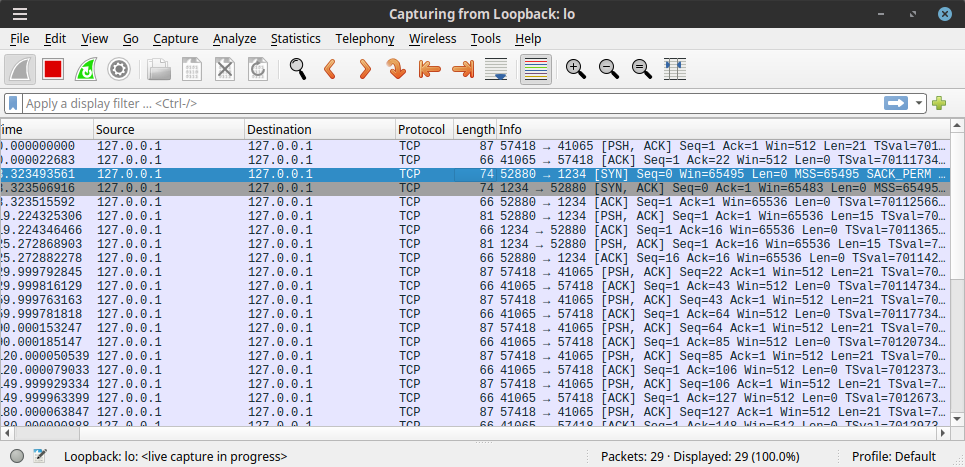
\includegraphics[scale=0.55]{res/7.wireshark-nc-chat.png}
\end{center}

\newpage

Wireshark позволяет полностью отследить всю переписку
\begin{center}
    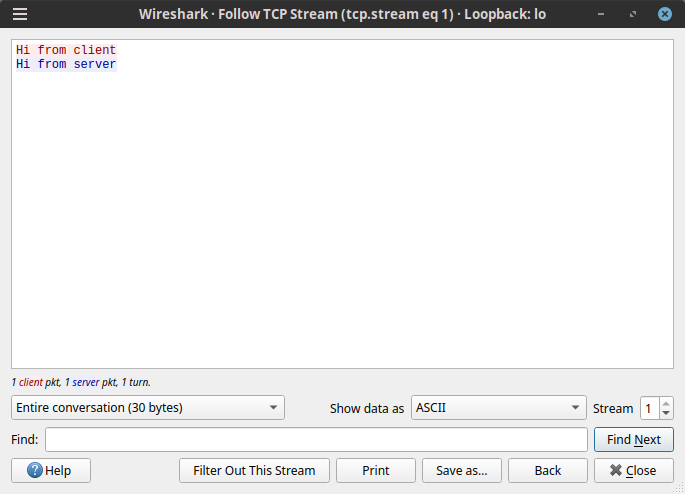
\includegraphics[scale=0.55]{res/7.wireshark-nc-follow.png}
\end{center}

\section*{3. Передача файлов}
\addcontentsline{toc}{section}{3. Передача файлов}

Все следующие примеры (включая сжатие) подразумевают не зашифрованную передачу, это значит Wireshark может перехватить и восстановить передаваемые файлы.

\subsection*{3.1 Передача одного файла}
\addcontentsline{toc}{subsection}{3.1 Передача одного файла}

На принимающей стороне, запускаем прослушивающий сервер \texttt{nc -nvlp 1234 > file.txt}.

Все параметры запуска уже были рассмотрены в предыдущем примере, вывод команды сделан в файл \texttt{file.txt}.

Получение файла
\begin{Verbatim}[frame=single,breaklines=true,breakanywhere=true]
    smart@thinkpad$ nc -nvlp 1234 > file.txt
    Connection from 127.0.0.1:56638
\end{Verbatim}

На передающей стороне, делаем такой вызов \texttt{cat file.txt | nc 127.0.0.1 1234}. В некоторых реализациях есть дополнительная опция \texttt{-q 0} для того, что бы netcat автоматически завершил работу сразу после отправки.

Передача файла
\begin{Verbatim}[frame=single,breaklines=true,breakanywhere=true]
    smart@thinkpad$ nc 127.0.0.1 1234 < file.txt

\end{Verbatim}

\subsection*{3.2 Передача одного файла с отображением прогресса}
\addcontentsline{toc}{subsection}{3.2 Передача одного файла с отображением прогресса}

Главный минус предыдущего подхода в том, что непонятно когда завершена передача.

Возможным решением может быть добавление счётчика на отправляющий и принимающей стороне.

Получение файла
\begin{Verbatim}[frame=single,breaklines=true,breakanywhere=true]
    smart@thinkpad$ nc -nvlp 1234 | pv -b > file.txt
    Connection from 127.0.0.1:36388
     304 B
\end{Verbatim}

Передача файла
\begin{Verbatim}[frame=single,breaklines=true,breakanywhere=true]
    smart@thinkpad$ cat file.txt | pv -b | nc 127.0.0.1 1234
    304 B
\end{Verbatim}

При помощи утилиты pv (pipeviewer) мы можем видеть прогресс передачи через подсчёт количества байт (ключ \texttt{-b} просто отображает итоговый объём, отключая анимацию передачи, хотя она бывает полезна при передаче больших объёмов).

\subsection*{3.3 Передача нескольких файлов}
\addcontentsline{toc}{subsection}{3.3 Передача нескольких файлов}

Для передачи нескольких файлов в одной директории можно написать простой bash-скрипт, который переберёт все файлы, и для каждого сделает вызод nc.

Другой вариант передачи -- запаковать её в тарбол на одном конце, и распаковать на другом. Кроме прочего, это позволит передать и права, выставленные на файлы.

Получение директории
\begin{Verbatim}[frame=single,breaklines=true,breakanywhere=true]
    smart@thinkpad$ nc -nvlp 1234 | pv -b | tar xf -
    Connection from 127.0.0.1:35942
    39.0MiB
\end{Verbatim}

Тут мы используем утилиту tar:

\begin{itemize}
    \item \texttt{x} -- производить операцию извлечения из обрабатываемого потока
    \item \texttt{f} -- обрабатывать архивный файл
    \item \texttt{-} -- вместо имени архива поток, полученный из пайпа
\end{itemize}

Передача директории
\begin{Verbatim}[frame=single,breaklines=true,breakanywhere=true]
    smart@thinkpad$ tar cf - . | pv -b | nc 127.0.0.1 1234
    39.0MiB
\end{Verbatim}

Тут мы используем утилиту tar:

\begin{itemize}
    \item \texttt{с} -- производить операцию сжатия
    \item \texttt{f} -- обрабатывать архивный файл
    \item \texttt{-} -- вместо файла, передаём данные в пайп
    \item \texttt{.} -- обрабатываем все файлы в текущей директории
\end{itemize}

\subsection*{3.4 Передача нескольких файлов со сжатием}
\addcontentsline{toc}{subsection}{3.4 Передача нескольких файлов со сжатием}

Для экономии трафика, можно сражу сжимать поток любым архиватором. Тема выбора подходящего архиватора для различных типов данных достойна отдельного исследования, мы будем использовать gzip, как оптимальное решение между скоростью работы, качеством сжатия и количеством потребляемых ресурсов. Для этого достаточно передать параметр \texttt{z} утилите tar.

Получение директории со сжатием
\begin{Verbatim}[frame=single,breaklines=true,breakanywhere=true]
    smart@thinkpad$ nc -nvlp 1234 | pv -b | tar xzf -
    Connection from 127.0.0.1:43324
    36.8MiB
\end{Verbatim}

Передача директории
\begin{Verbatim}[frame=single,breaklines=true,breakanywhere=true]
    smart@thinkpad$ tar czf - . | pv -b | nc 127.0.0.1 1234
    36.8MiB
\end{Verbatim}

Удалось уменьшить объём передаваемого трафика с 39.0MiB до 36.8MiB (экономия больше 5\%!).

\subsection*{3.5 Передача образа жёского диска}
\addcontentsline{toc}{subsection}{3.5 Передача образа жёского диска}

Иногда необходимо сделать резервную копию образа жёсткого диска с одной машины на другую.

В таком случае, для отправки образа можно использовать такую команду \texttt{bzip2 -c /dev/sdb1 | nc -nvlp 1234}. Эта команда будет пересылать все данные с диска \texttt{/dev/sdb1}. Учитывая, что мы читаем диск как набор секторов (в двоичном формате), для сжатия будем использовать \texttt{bzip2}.

Со стороны получателя, будет распаковывать поток и складывать в отдельный файл \texttt{nc 192.168.1.102 1234 | pv -b | bzip2 -d > hdImage.img}

\section*{4. Защищенное взаимодействие}
\addcontentsline{toc}{section}{4. Защищенное взаимодействие}

\subsection*{4.1 Установка cryptcat}
\addcontentsline{toc}{subsection}{4.1 Установка cryptcat}

Утилита cryptcat довольно специфичная. Её нет в стандартном репозитории для моего дистрибутива linux (Arch linux) и нет а пользовательских пакетах (AUR). Дистрибутив Kali linux использует довольно старую версию пакета (\texttt{20031202}), но на официальном сайте (\url{https://cryptcat.sourceforge.net/}) есть ссылка на sourceforge, где размещена версия от октября 2005-го года.

Берём исходники утилиты по ссылке
\url{https://sourceforge.net/projects/cryptcat/files/cryptcat-unix-1.2/cryptcat-unix-1.2.1/cryptcat-unix-1.2.1.tar/download}

Изучение исходников показывает, что по сути это старая версия утилиты Netcat для которой имплантирован модуль twofish2. Примечания к релизу содержат некоторое количество известных багов, которые планируется решить когда-то в будущем.

Сборка из исходников сыпет большим количеством предупреждений, т.к. код был написан на более старую версию API glibc.

\subsection*{4.2 Взаимодействие процессов}
\addcontentsline{toc}{subsection}{4.2 Взаимодействие процессов}

Повторим эксперимент с созданием чата.

Запуск сервера и общение с клиентом
\begin{Verbatim}[frame=single,breaklines=true,breakanywhere=true]
    smart@thinkpad$ ./cryptcat -nvlp 1234
    listening on [any] 1234 ...
    connect to [127.0.0.1] from (UNKNOWN) [127.0.0.1] 39944
    hello from client
    hello from server
\end{Verbatim}

Запуск клиента и общение с сервером
\begin{Verbatim}[frame=single,breaklines=true,breakanywhere=true]
    smart@thinkpad$ ./cryptcat 127.0.0.1 1234
    hello from client
    hello from server
\end{Verbatim}

Проверка состояние сокета
\begin{Verbatim}[frame=single,breaklines=true,breakanywhere=true]
    smart@thinkpad$ ss -tp | grep nc
    ESTAB 0   0      127.0.0.1:39944          127.0.0.1:search-agent users:(("cryptcat",pid=71954,fd=3))
    ESTAB 0   0      127.0.0.1:search-agent   127.0.0.1:39944        users:(("cryptcat",pid=71953,fd=4))
\end{Verbatim}

\newpage

Пакеты, пойманные Wireshark
\begin{center}
    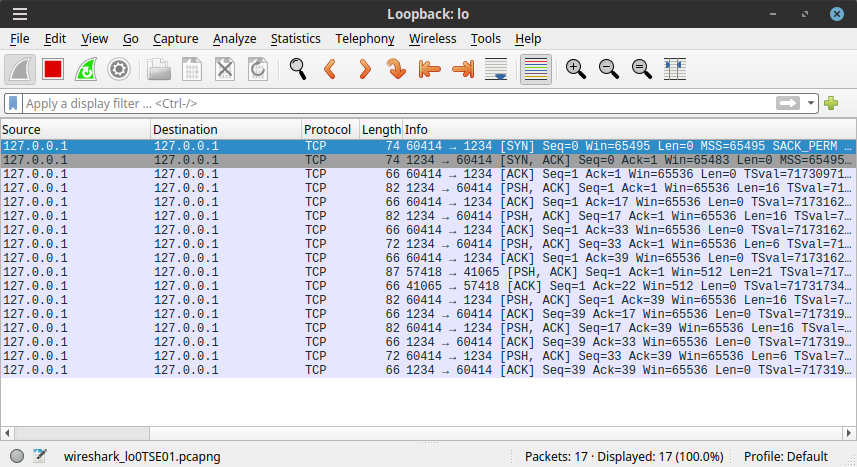
\includegraphics[scale=0.55]{res/7.wireshark-cryptcat-chat.png}
\end{center}

Wireshark показывает, что данные переданы в зашифрованном виде
\begin{center}
    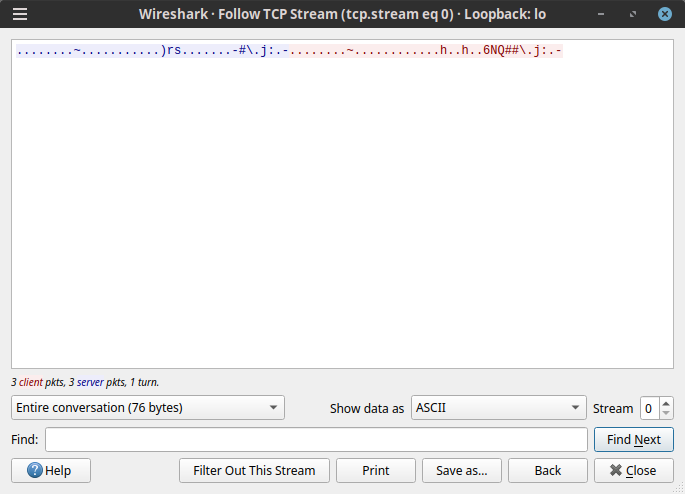
\includegraphics[scale=0.55]{res/7.wireshark-cryptcat-follow.png}
\end{center}

\subsection*{4.3 Передача файлов}
\addcontentsline{toc}{subsection}{4.3 Передача файлов}

Передача файлов работает аналогично Netcat, данные зашифрованы.

Получение файла
\begin{Verbatim}[frame=single,breaklines=true,breakanywhere=true]
    smart@thinkpad$ ../cryptcat -nvlp 1234 | pv -b > file.txt
    listening on [any] 1234 ...
    connect to [127.0.0.1] from (UNKNOWN) [127.0.0.1] 54856
    304 B
\end{Verbatim}

Передача файла
\begin{Verbatim}[frame=single,breaklines=true,breakanywhere=true]
    smart@thinkpad$ cat file.txt | pv -b | ./cryptcat 127.0.0.1 1234
    304 B
\end{Verbatim}

\section*{5. Direct Network Traffic}
\addcontentsline{toc}{section}{5. Direct Network Traffic}

Выполним установку двунаправленного пайпа для редиректа локального порта 1234 на 80-й порт google.

Для начала определим, что должно получиться в итоге. При запросе на 80-й порт, google отвечает 301 и отправляет устанавливать https соединение. Но даже такого ответа нам достаточно для теста.

\begin{Verbatim}[frame=single,breaklines=true,breakanywhere=true]
    smart@thinkpad$ curl google.com
    <HTML><HEAD><meta http-equiv="content-type" content="text/html;charset=utf-8">
    <TITLE>301 Moved</TITLE></HEAD><BODY>
    <H1>301 Moved</H1>
    The document has moved
    <A HREF="http://www.google.com/">here</A>.
    </BODY></HTML>
\end{Verbatim}

Подготовм двунаправленный пайп.
\texttt{nc -l -p 1233 | nc www.google.com 80 | nc -l -p 1234}

После этого, через curl вначале сделаем запрос на порт 1233, потом прочитаем ответ с порта 1234.

Результат работы пайпа
\begin{Verbatim}[frame=single,breaklines=true,breakanywhere=true]
    smart@thinkpad$ nc -lp 1233 | nc google.com 80 | nc -lp 1234
    GET / HTTP/1.1
    Host: 127.0.0.1:1234
    User-Agent: curl/7.87.0
    Accept: */*
\end{Verbatim}

Результат работы curl
\begin{Verbatim}[frame=single,breaklines=true,breakanywhere=true]
    smart@thinkpad$ curl 127.0.0.1:1233
    ^[[A^C
    smart@thinkpad$ curl 127.0.0.1:1234
    <HTML><HEAD><meta http-equiv="content-type" content="text/html;charset=utf-8">
    <TITLE>301 Moved</TITLE></HEAD><BODY>
    <H1>301 Moved</H1>
    The document has moved
    <A HREF="http://www.google.com:1233/">here</A>.
    </BODY></HTML>
\end{Verbatim}

Естественно, весь трафик ходит незащищенным.

\section*{Выводы}
\addcontentsline{toc}{section}{Выводы}

В этой работе мы познакомились с возможностями утилиты netcat и её безопасной (но, не поддерживаемой) версии cryptcat.

С практической точки зрения, для передачи файлов удобнее использовать rsync (он безопасный и имеет множество полезных опеций), безопасно туннелировать трафик можно при помощи ssh, а локальный редирект портов можно осуществлять средствами встроенного фаервола.
%\input{text}                                 % inclide the main text
%% \newpage
\section*{}
\addcontentsline{toc}{section}{List of sources}

\begin{thebibliography}{00}

% Use: \cite{label1}
\bibitem{label1} JavaScript.ru: Справочник по работе с WebSocket. URL: https://learn.javascript.ru/websockets (дата обращения: 16.04.2023).

\bibitem{label2} Internet Engineering Task Force (IETF) / Request for Comments: 6455: The WebSocket Protocol (December 2011). URL: https://datatracker.ietf.org/doc/html/rfc6455 (дата обращения: 20.04.2023).

\bibitem{label3} MDN Web Docs / The WebSocket API (WebSockets). URL: https://developer.mozilla.org/en-US/docs/Web/API/WebSockets\_API (дата обращения: 20.04.2023).

\bibitem{label4} Nginx blog / NGINX as a WebSocket Proxy (Rick Nelson, 2014). URL: https://www.nginx.com/blog/websocket-nginx/ (дата обращения: 23.04.2023).

\bibitem{label5} How to scale WebSocket – horizontal scaling with WebSocket tutorial (2020). URL: https://tsh.io/blog/how-to-scale-websocket/ (дата обращения: 26.04.2023).

\end{thebibliography}                              % inclide the list of sources


\end{document}

%------------------------------------------------------------------------------
% Examples:
%
%
%
% \begin{figure}[H]
% \centering
% \includegraphics[scale=0.8]{res/pic01}
% \caption{Picture description}
% \end{figure}
%
%
%
% \begin{table}[htb]
%     \begin{tabularx}{\textwidth}{|X|c|c|c|c|c|}
%     \hline
%     \multirow{2}{*}{tb1} & \multirow{2}{*}{tbl2} & \multicolumn{4}{c|}{tbl3} \\
%     \cline{3-6}
%     {} & {} & A & B & C & D\\
%     \hline
%     Text & {} & Text & {} & {} & {} \\
%     \hline
%     \end{tabularx}
% \caption{Table description}
% \end{table}